%%%%%%%%%%%%%%%%%%%%%%%%%%%%%%%%%%%%%
% Check out the accompanying book, Even Better Books with LaTeX the Agile Way in 2023, for a discussion of the template and step-by-step instructions. https://amzn.to/3HqwgXM https://leanpub.com/eBBwLtAW/
% The template was originally created by Clemens Lode, LODE Publishing (www.lode.de), on 1/1/2023. Feel free to use this template for your book project!
% I would be happy if you included a short mention in your book in order to help others to create their own books, too ("Book template based on \textit{Even Better Books with LaTeX the Agile Way in 2023} by Clemens Lode").
% Contact me at mail@lode.de if you need help with the template or are interested in our editing and publishing services.
% And don't forget to follow us on Instagram! https://www.instagram.com/lodepublishing/ https://www.instagram.com/betterbookswithlatex/
%%%%%%%%%%%%%%%%%%%%%%%%%%%%%%%%%%%%%

% To create an EPUB file, select pdfLaTeX in the Menu in the top-left and choose the conversion method in the /latexmkrc file.

% Select document class scrbook to be in the two-page mode and accommodate for the binding of a printed book.
% The bibliography receives an entry in the table of contents but no number.
\documentclass[
    pagesize=auto,
    bibliography=totocnumbered,
    cleardoublepage=empty,
    paper=5in:8in,
    DIV=calc,            % let KOMA compute a good type area
    headings=small,      % smaller chapter/section defaults
    numbers=noendperiod  % aesthetic preference
]{scrbook}

%%%%%%%%%%%%%%%%%%%%%%%%%%%%%%%%%%%%%
% Check out the accompanying book, Even Better Books with LaTeX the Agile Way in 2023, for a discussion of the template and step-by-step instructions. https://amzn.to/3HqwgXM https://leanpub.com/eBBwLtAW/
% The template was originally created by Clemens Lode, LODE Publishing (www.lode.de), on 1/1/2023. Feel free to use this template for your book project!
% I would be happy if you included a short mention in your book in order to help others to create their own books, too ("Book template based on \textit{Even Better Books with LaTeX the Agile Way in 2023} by Clemens Lode").
% Contact me at mail@lode.de if you need help with the template or are interested in our editing and publishing services.
% And don't forget to follow us on Instagram! https://www.instagram.com/lodepublishing/ https://www.instagram.com/betterbookswithlatex/
%%%%%%%%%%%%%%%%%%%%%%%%%%%%%%%%%%%%%

% Replace "The Title" with your book title.
\newcommand{\mytitle}{The Title}

% Replace "The subtitle" with your book's subtitle.
\newcommand{\mysubtitle}{The subtitle}

% Replace "Publishing Company" with the name of the publishing company it is published.
\newcommand{\mypublishingcompany}{Daniel Díaz Quílez}

% Replace "Location of the Publishing Company (city)" with the location (e.g., the city) of the publishing company.
\newcommand{\mypublishingcompanylocation}{Helsinki, Finlandia}

\newcommand{\mypublishingcompanyurl}{\url{https://www.lode.de}}


% Upload a low-resolution jpg (e-book) and a high-resolution (pdf/print) png version of your front cover into the "images" folder. If you need help with creating a cover, email us at mail@lode.de to talk about what you need, and we will do our best to help you.
\newcommand{\coverImage}{images/cover.jpg}
\newcommand{\hiresCoverImage}{images/cover.png}


% Replace "Your email address" with your email address.
% Replace "Edition" with the edition number.
% Replace the ISBNs with your ISBNs.
% Replace "Your editor's name" with your editor's name.
% Replace "Your designer's name" with your book cover designer's name.
% Replace "Your image sources" with the sources of your images (including icons) and relevant license information.
% Replace "Your newsletter email" with your newsletter email.
% Replace "Your newsletter URL" with your website's newsletter URL.


\newcommand{\mypublishingcompanyemail}{Your email address}
\newcommand{\editionNumber}{First}

% Buy ISBNs or use the ISBNs generated by Amazon and list them  here.
\newcommand{\ebookISBN}{123-4-567890-12-3}
\newcommand{\softcoverISBN}{123-4-567890-12-4}
\newcommand{\hardcoverISBN}{123-4-567890-12-5}

\newcommand{\editorName}{Daniel Díaz Quílez}
\newcommand{\designerName}{Daniel Díaz Quílez}
\newcommand{\typesetterName}{Daniel Díaz Quílez}
\newcommand{\imageSources}{Daniel Díaz Quílez}

\newcommand{\newsletterMail}{Your newsletter email}
\newcommand{\newsletterURL}{Your newsletter URL}

% If you want to subscribe to this book's newsletter, write an email to newsletter@lode.de or follow us on Instagram.com/lodepublishing or Instagram/betterbookswithlatex

\newcommand{\yourName}{Your name}

% Replace city, country, and date with the place and country where you (or your company) are located and the date when the preface was finished (it does not have to be the release date of the book).

\newcommand{\yourCity}{Your city}
\newcommand{\yourCountry}{Your country}
\newcommand{\prefaceDate}{\today}

\newif\ifuseAuthorImage
% Uncomment and upload author images
%\useAuthorImagetrue

\ifuseAuthorImage
    \newcommand{\authorImage}{images/author.jpg}
    \newcommand{\authorImageHiRes}{images/author.png}
\fi


% Uncomment \seriestrue if your book is part of a series.
\newif\ifseries
%\seriestrue

\ifseries
% Replace "Title of Book Series" with the title of the book series.
% Replace "Title of Part One" with the title of part one.
% Replace "Title of Part Two" with the title of part two.
% Replace "Title of Part Three" with the title of part three, or remove the line if there is no part three.
% Replace "Title of Part Four" with the title of part four, or remove the line if there is no part four.

\newcommand{\partOneTitle}{Title of Part One}
\newcommand{\partTwoTitle}{Title of Part Two}
\newcommand{\partThreeTitle}{Title of Part Three}
\newcommand{\partFourTitle}{Title of Part Four}

\newcommand{\titleOfTheBookSeries}{Title of the Book Series}

\newif\firstBookOfSeries
\firstBookOfSeries

\ifFirstBookOfSeries
\else
\newcommand{\partPreviousPart}{Number of the previous part in the book series}
\newcommand{\titlePreviousPart}{Title of the previous part in the book series}

\newcommand{\previousCoverImage}{images/previous_part_of_the_series_Cover.jpg}
\newcommand{\previousCoverImageHiRes}{images/previous_part_of_the_series_Cover_hires.png}

\fi


% If you want a different size than 6"x9", change the lib/bookformat.tex file accordingly.

\newif\ifhardcover
% Uncomment for selecting hardcover.
%\hardcovertrue

\title{\mytitle}

% Load additional LaTeX libraries.
%%%%%%%%%%%%%%%%%%%%%%%%%%%%%%%%%%%%% 
% Check out the accompanying book, Even Better Books with LaTeX the Agile Way in 2023, for a discussion of the template and step-by-step instructions. https://amzn.to/3HqwgXM https://leanpub.com/eBBwLtAW/
% The template was originally created by Clemens Lode, LODE Publishing (www.lode.de), on 1/1/2023. Feel free to use this template for your book project! 
% I would be happy if you included a short mention in your book in order to help others to create their own books, too ("Book template based on \textit{Even Better Books with LaTeX the Agile Way in 2023} by Clemens Lode").
% Contact me at mail@lode.de if you need help with the template or are interested in our editing and publishing services.
% And don't forget to follow us on Instagram! https://www.instagram.com/lodepublishing/ https://www.instagram.com/betterbookswithlatex/
%%%%%%%%%%%%%%%%%%%%%%%%%%%%%%%%%%%%%



% This configures the PDF/EPUB output.
%%%%%%%%%%%%%%%%%%%%%%%%%%%%%%%%%%%%% 
% Check out the accompanying book, Even Better Books with LaTeX the Agile Way in 2023, for a discussion of the template and step-by-step instructions. https://amzn.to/3HqwgXM https://leanpub.com/eBBwLtAW/
% The template was originally created by Clemens Lode, LODE Publishing (www.lode.de), on 1/1/2023. Feel free to use this template for your book project! 
% I would be happy if you included a short mention in your book in order to help others to create their own books, too ("Book template based on \textit{Even Better Books with LaTeX the Agile Way in 2023} by Clemens Lode").
% Contact me at mail@lode.de if you need help with the template or are interested in our editing and publishing services.
% And don't forget to follow us on Instagram! https://www.instagram.com/lodepublishing/ https://www.instagram.com/betterbookswithlatex/
%%%%%%%%%%%%%%%%%%%%%%%%%%%%%%%%%%%%%

% This command enables checking if XeLaTeX is used.
\usepackage{ifxetex}

\ifxetex
    % For the PDF output, load the following additional packages.
    
    % This adjusts figures to fit into the width of a page.
    \usepackage{adjustbox}
    
    % Use this for fancy lines at the beginning of chapters and the end of sections.
    \usepackage{psvectorian} 

\else
    % Ignore adjustbox commands (HTML files do not have a width).
    \newcommand{\adjustbox}[2][]{#1}

    % Ignore psvectorian lines.
    \newcommand{\psvectorian}[2][]{}
\fi

% Translate newpage and hrule commands.
\ifx\HCode\undefined
    \newcommand{\nextpage}[1][]{}
\else
    \newcommand{\nextpage}[1][]{\HCode{<mbp:pagebreak />}}
    \renewcommand{\hrule}{\HCode{<hr style="clear: both" />}}
\fi

% Sets up support for multiple languages.
%%%%%%%%%%%%%%%%%%%%%%%%%%%%%%%%%%%%%
% Check out the accompanying book, Even Better Books with LaTeX the Agile Way in 2023, for a discussion of the template and step-by-step instructions. https://amzn.to/3HqwgXM https://leanpub.com/eBBwLtAW/
% The template was originally created by Clemens Lode, LODE Publishing (www.lode.de), on 1/1/2023. Feel free to use this template for your book project!
% I would be happy if you included a short mention in your book in order to help others to create their own books, too ("Book template based on \textit{Even Better Books with LaTeX the Agile Way in 2023} by Clemens Lode").
% Contact me at mail@lode.de if you need help with the template or are interested in our editing and publishing services.
% And don't forget to follow us on Instagram! https://www.instagram.com/lodepublishing/ https://www.instagram.com/betterbookswithlatex/
%%%%%%%%%%%%%%%%%%%%%%%%%%%%%%%%%%%%%

% Activate American language (and \babelEN).
% \usepackage[american]{babel}

% Activate Spanish language (and \babelES).
\usepackage[spanish]{babel}

% Activate German language (and \babelDE).
%\usepackage[ngerman]{babel}

% Fix PDF creation.
\ifxetex
	\let\pdfstrcmp\strcmp
\fi
% Set up macros to support multiple languages:
\newcommand{\babelES}[1]{\ifnum\pdfstrcmp{\languagename}{spanish}=0 {#1}\fi}
\newcommand{\babelDE}[1]{\ifnum\pdfstrcmp{\languagename}{ngerman}=0 {#1}\fi}
\newcommand{\babelEN}[1]{\ifnum\pdfstrcmp{\languagename}{american}=0 {#1}\fi}

\addto\captionsspanish{%
  \renewcommand{\contentsname}{Índice}%
}


% Loads packages to be able to configure hyphenation.
%%%%%%%%%%%%%%%%%%%%%%%%%%%%%%%%%%%%% 
% Check out the accompanying book, Even Better Books with LaTeX the Agile Way in 2023, for a discussion of the template and step-by-step instructions. https://amzn.to/3HqwgXM https://leanpub.com/eBBwLtAW/
% The template was originally created by Clemens Lode, LODE Publishing (www.lode.de), on 1/1/2023. Feel free to use this template for your book project! 
% I would be happy if you included a short mention in your book in order to help others to create their own books, too ("Book template based on \textit{Even Better Books with LaTeX the Agile Way in 2023} by Clemens Lode").
% Contact me at mail@lode.de if you need help with the template or are interested in our editing and publishing services.
% And don't forget to follow us on Instagram! https://www.instagram.com/lodepublishing/ https://www.instagram.com/betterbookswithlatex/
%%%%%%%%%%%%%%%%%%%%%%%%%%%%%%%%%%%%%

% Use fontenc to properly hyphenate accented languages.
\usepackage[T1]{fontenc}

% Add a list of words to enforce a certain hyphenation for them.
\usepackage{hyphenat}
\hyphenation{}



% In this package, we define the dimensions of the printed book.
%%%%%%%%%%%%%%%%%%%%%%%%%%%%%%%%%%%%%
% Check out the accompanying book, Even Better Books with LaTeX the Agile Way in 2023, for a discussion of the template and step-by-step instructions. https://amzn.to/3HqwgXM https://leanpub.com/eBBwLtAW/
% The template was originally created by Clemens Lode, LODE Publishing (www.lode.de), on 1/1/2023. Feel free to use this template for your book project!
% I would be happy if you included a short mention in your book in order to help others to create their own books, too ("Book template based on \textit{Even Better Books with LaTeX the Agile Way in 2023} by Clemens Lode").
% Contact me at mail@lode.de if you need help with the template or are interested in our editing and publishing services.
% And don't forget to follow us on Instagram! https://www.instagram.com/lodepublishing/ https://www.instagram.com/betterbookswithlatex/
%%%%%%%%%%%%%%%%%%%%%%%%%%%%%%%%%%%%%

%%%%%%%%%%%%%%%%%
% Configure bleed.
%%%%%%%%%%%%%%%%%

% If your book includes images that extend beyond the usual margins, set bleed to 0.125in and activate the corresponding option in Amazon KDP.

\newcommand{\margintop}{1.65cm}
\newcommand{\marginbottom}{2.0cm}
\newcommand{\marginoutside}{1.5cm}

%%%%%%%%%%%%%%%%%
% The inner margins depend on the number of pages of your book.
%%%%%%%%%%%%%%%%%

% Note that books printed by Amazon have an upper limit of number of pages. This limits depends on your book's dimensions, whether it is a paperback or hardcover format, and whether it is printed in black and white or in color.
% See https://kdp.amazon.com/en_US/help/topic/GVBQ3CMEQW3W2VL6

% Select the margin for 24 - 150 pages by default.
\newcommand{\margininside}{1.5cm}

%%%%%%%%%%%%%%%%%
% Hardcover / Softcover Formats. Selecting one of these ensures that you can use the same PDF for hardcover and softcover books on Amazon.
%%%%%%%%%%%%%%%%%

% Select 5x8 by default.
\newcommand{\bookwidth}{5in}
\newcommand{\bookheight}{8in}

%%%%%%%%%%%%%%%%%
% Hardcover-only formats. Selecting one of these requires you to create a separate PDF for a softcover version.
%%%%%%%%%%%%%%%%%

%\newcommand{\bookwidth}{8.25in}\newcommand{\bookheight}{11in}

%%%%%%%%%%%%%%%%%
% Softcover-only formats. Selecting one of these requires you to create a separate PDF for a hardcover version.
%%%%%%%%%%%%%%%%%

%\newcommand{\bookwidth}{5in}\newcommand{\bookheight}{8in}
%\newcommand{\bookwidth}{5.25in}\newcommand{\bookheight}{8in}
%\newcommand{\bookwidth}{5.06in}\newcommand{\bookheight}{7.81in}
%\newcommand{\bookwidth}{6.69in}\newcommand{\bookheight}{9.61in}
%\newcommand{\bookwidth}{7.44in}\newcommand{\bookheight}{9.69in}
%\newcommand{\bookwidth}{7.5in}\newcommand{\bookheight}{9.25in}
%\newcommand{\bookwidth}{8in}\newcommand{\bookheight}{10in}
%\newcommand{\bookwidth}{8.5in}\newcommand{\bookheight}{11in}

%%%%%%%%%%%%%%%%%
% And now we are putting everything together to set the dimensions of the book.
%%%%%%%%%%%%%%%%%

\usepackage[
    paperwidth=\bookwidth,
    paperheight=\bookheight,
    inner=\margininside,
    outer=\marginoutside,
    top=\margintop,
    bottom=\marginbottom,
    includehead,
    includefoot,
    headheight=0pt,
    bindingoffset=6mm
]{geometry}


% This package defines all the box commands.
%%%%%%%%%%%%%%%%%%%%%%%%%%%%%%%%%%%%% 
% Check out the accompanying book, Even Better Books with LaTeX the Agile Way in 2023, for a discussion of the template and step-by-step instructions. https://amzn.to/3HqwgXM https://leanpub.com/eBBwLtAW/
% The template was originally created by Clemens Lode, LODE Publishing (www.lode.de), on 1/1/2023. Feel free to use this template for your book project! 
% I would be happy if you included a short mention in your book in order to help others to create their own books, too ("Book template based on \textit{Even Better Books with LaTeX the Agile Way in 2023} by Clemens Lode").
% Contact me at mail@lode.de if you need help with the template or are interested in our editing and publishing services.
% And don't forget to follow us on Instagram! https://www.instagram.com/lodepublishing/ https://www.instagram.com/betterbookswithlatex/
%%%%%%%%%%%%%%%%%%%%%%%%%%%%%%%%%%%%%

% Replace the "Did you know?", "Read more in...", box titles, and icons if necessary.

% Configuring the commands for the PDF output...
\ifx\HCode\undefined 

    % If you want to add a picture to the top right corner of a box, uncomment the line and upload the picture.

    \usepackage[many]{tcolorbox}
    
    \newtcolorbox{problem}[1][]{colframe = black!30,colback  = black!4,coltitle = black!20!black,title=\babelDE{\textbf{Frage}}\babelEN{\textbf{Question}}
    %\hfill\smash{\raisebox{-11pt}{\includegraphics[height=1cm]{images/speech-bubble-cloud-with-question-mark.png}}}
    , #1,}
    
    \newtcolorbox{idea}[1][]{colframe = black!30,colback  = black!5,coltitle = black!30!black,title=\babelDE{\textbf{Idee}}\babelEN{\textbf{Idea}}
    %\hfill\smash{\raisebox{-11pt}{\includegraphics[height=1cm]{images/lightbulb-idea}}}
    , #1,}

    \newtcolorbox{example}[1][]{colframe = black!20,colback  = black!0,coltitle = black!20!black,title=\babelDE{\textbf{Beispiel}}\babelEN{\textbf{Example}}
    %\hfill\smash{\raisebox{-11pt}{\includegraphics[height=1cm]{images/book-and-test-tube-with-supporter}}}
    , #1,}

    
    \newtcolorbox{biography}[2][]{colframe = black!30,colback  = black!5,coltitle = black!30!black,title=\babelDE{Biographie -- }\babelEN{Biography---}\textbf{#2}
    %\hfill\smash{\raisebox{-11pt}{\includegraphics[height=1cm]{images/identity-card}}}
    , #1,}
    
% ... and for the HTML output.
\else
	
    \newenvironment{problem}[1][]{\bfseries\HCode{<b>}}{\HCode{</b>}\par}
    
    \newenvironment{idea}[1][]{\bfseries\HCode{<b>}}{\HCode{</b>}\par}
	
    \newenvironment{example}[1][]{\hrule\par \textbf{\babelDE{Beispiel}\babelEN{Example}}\par}{\hrule\par}
    
    \newenvironment{biography}[2][]{\hrule\par\textbf{\babelDE{Biographie}\babelEN{Biography}} \emdash \textbf{#2}\par}{\hrule\par}

\fi



% Print out listings as-is (ignoring any special characters).
\usepackage{listings}




\ifx\HCode\undefined 

% This code loads the \leftbar command for the definition environment.
    \usepackage{framed}
    \newenvironment{definition}[2][]{\begin{leftbar}\textbf{\textsc{#2}}\ ·\ #1}{\end{leftbar}\vspace{-\baselineskip}}


% Create a new environment "myquotation" that indents a whole paragraph to show that it is not part of the normally flowing text.
    \renewcommand{\indent}{\begin{picture}(0,0)\put(10,-5){\makebox(0,0){\scalebox{6}{\textcolor{lightgray}{``}}}}\end{picture}\hspace*{1.0cm}\hangindent=1.15cm}
    \newenvironment{myquotation}{\indent}{}

\else
    \newenvironment{definition}[2][]{\textbf{\textsc{#2}}\ ·\ #1}

% For the HTML output for the e-book, the indentation is defined in the style.css.
    \newenvironment{myquotation}
    {\begin{quotation}}{\end{quotation}}

    
\fi



% Uncomment this command for more error and warning messages.
%%%%%%%%%%%%%%%%%%%%%%%%%%%%%%%%%%%%%% 
% Check out the accompanying book, Even Better Books with LaTeX the Agile Way in 2023, for a discussion of the template and step-by-step instructions. https://amzn.to/3HqwgXM https://leanpub.com/eBBwLtAW/
% The template was originally created by Clemens Lode, LODE Publishing (www.lode.de), on 1/1/2023. Feel free to use this template for your book project! 
% I would be happy if you included a short mention in your book in order to help others to create their own books, too ("Book template based on \textit{Even Better Books with LaTeX the Agile Way in 2023} by Clemens Lode").
% Contact me at mail@lode.de if you need help with the template or are interested in our editing and publishing services.
% And don't forget to follow us on Instagram! https://www.instagram.com/lodepublishing/ https://www.instagram.com/betterbookswithlatex/
%%%%%%%%%%%%%%%%%%%%%%%%%%%%%%%%%%%%%


% Activate warnings about outdated/invalid packages.
\RequirePackage[l2tabu, orthodox]{nag}

% Configure LaTeX to provide full error messages.
\errorcontextlines 10000

% Loading this package sets up a balanced multicol environment that can end mid-page (needs to be loaded before fonts because of imakeidx package).
%%%%%%%%%%%%%%%%%%%%%%%%%%%%%%%%%%%%% 
% Check out the accompanying book, Even Better Books with LaTeX the Agile Way in 2023, for a discussion of the template and step-by-step instructions. https://amzn.to/3HqwgXM https://leanpub.com/eBBwLtAW/
% The template was originally created by Clemens Lode, LODE Publishing (www.lode.de), on 1/1/2023. Feel free to use this template for your book project! 
% I would be happy if you included a short mention in your book in order to help others to create their own books, too ("Book template based on \textit{Even Better Books with LaTeX the Agile Way in 2023} by Clemens Lode").
% Contact me at mail@lode.de if you need help with the template or are interested in our editing and publishing services.
% And don't forget to follow us on Instagram! https://www.instagram.com/lodepublishing/ https://www.instagram.com/betterbookswithlatex/
%%%%%%%%%%%%%%%%%%%%%%%%%%%%%%%%%%%%%

% Balance the contents of two columns (as opposed to filling first the left column and then the right). This is used for the glossary.
% See https://tex.stackexchange.com/questions/241094/multicol-column-balancing-only-after-a-minimum-number-of-lines

\ifxetex
\usepackage[balancingshow]{multicol}
\usepackage{regexpatch}

\newcounter{multicolminlines}
\setcounter{multicolminlines}{1}

\makeatletter
\xpatchcmd\balance@columns
   {\ifnum\dimen@<\topskip
     \mult@info\@ne
       {Start value
          \the\dimen@  \space ->
          \the\topskip \space (corrected)}%
     \dimen@\topskip
   \fi}
   {\skip@\c@multicolminlines\baselineskip
   \advance\skip@-\baselineskip
   \advance\skip@\topskip
   \ifnum\dimen@<\skip@
     \mult@info\@ne
       {Start value
          \the\dimen@  \space ->
          \the\skip@ \space (corrected)}%
     \dimen@\skip@
   \fi
   }
   {\typeout{Success!}}{\patchFAILED}
\makeatother
\else

    \newenvironment{multicols}[2][]{}{}

\fi


% Loads the bibliography support and the bibliography files.
%%%%%%%%%%%%%%%%%%%%%%%%%%%%%%%%%%%%%
% Check out the accompanying book, Even Better Books with LaTeX the Agile Way in 2023, for a discussion of the template and step-by-step instructions. https://amzn.to/3HqwgXM https://leanpub.com/eBBwLtAW/
% The template was originally created by Clemens Lode, LODE Publishing (www.lode.de), on 1/1/2023. Feel free to use this template for your book project!
% I would be happy if you included a short mention in your book in order to help others to create their own books, too ("Book template based on \textit{Even Better Books with LaTeX the Agile Way in 2023} by Clemens Lode").
% Contact me at mail@lode.de if you need help with the template or are interested in our editing and publishing services.
% And don't forget to follow us on Instagram! https://www.instagram.com/lodepublishing/ https://www.instagram.com/betterbookswithlatex/
%%%%%%%%%%%%%%%%%%%%%%%%%%%%%%%%%%%%%

%%%%%%%%%%%%%%%%%
% Set up the bibliography.
%%%%%%%%%%%%%%%%%


\ifxetex
% See https://www.ctan.org/pkg/biblatex for documentation.
	\usepackage[indexing=cite,style=authoryear,sortlocale=de_DE,natbib=true]{biblatex}
\else
	\usepackage{natbib}
	\usepackage{usebib}

	% \citetitle does not work with natbib / pdfLaTeX -> translate into \usebibentry
	\newcommand{\citetitle}[2][]{\textit{\usebibentry{#2}{title}}}
\fi

% Load the corresponding bibliography files.
\ifxetex
	\babelEN{\addbibresource{chapters/bibliography/english.bib}}
\else
    \babelEN{\bibinput{chapters/bibliography/english}}
\fi


% Add a command to allow a preface for the bibliography (optional).
\newcommand{\bibpreface}[1]{\patchcmd{\thebibliography}{\list}{#1\list}{}{}}



% Use csquotes to correctly typeset quoted text according to the selected language.
\usepackage{csquotes}


% Write the name of a referenced section or chapter label with \nameref{label}.
\usepackage{nameref}
\newcommand{\reference}[2][]{see \nameref{#2}, Chapter~\ref{#2}}


% This package loads and configures the fonts we use.
%%%%%%%%%%%%%%%%%%%%%%%%%%%%%%%%%%%%%
% Check out the accompanying book, Even Better Books with LaTeX the Agile Way in 2023, for a discussion of the template and step-by-step instructions. https://amzn.to/3HqwgXM https://leanpub.com/eBBwLtAW/
% The template was originally created by Clemens Lode, LODE Publishing (www.lode.de), on 1/1/2023. Feel free to use this template for your book project!
% I would be happy if you included a short mention in your book in order to help others to create their own books, too ("Book template based on \textit{Even Better Books with LaTeX the Agile Way in 2023} by Clemens Lode").
% Contact me at mail@lode.de if you need help with the template or are interested in our editing and publishing services.
% And don't forget to follow us on Instagram! https://www.instagram.com/lodepublishing/ https://www.instagram.com/betterbookswithlatex/
%%%%%%%%%%%%%%%%%%%%%%%%%%%%%%%%%%%%%


% Set font size of captions to small.
\ifxetex
    \usepackage[labelfont=bf]{caption}
    \captionsetup{font=small}
\fi

% Use this shorter command for textemdash.
\newcommand{\emdash}[1][]{\textemdash}

% Set bibliography to footnote size.
\renewcommand{\bibfont}{\footnotesize}
% You can use ``same'' (same font as your document's), ``sf'', ``tt''  or ``rm'' for monospaced font. Also see https://www.ctan.org/pkg/url
\usepackage{url}
\urlstyle{same}

%-------------------------------------------
% Create hyperlinks within PDF files but do not mark them as links.
\ifxetex
    \usepackage{hyperref}[2011/02/05]
    \hypersetup{hidelinks}
\fi

% The following commands improve the font face for the PDF output (font tweaks are not available for e-books).
\ifxetex
% Prevent splitting footnotes over several pages. See https://texfaq.org/FAQ-splitfoot
    \interfootnotelinepenalty=10000

% Set the footnote font size to very small.
    \renewcommand{\footnotesize}{\scriptsize}


% Set the font size of the index to very small.
    \usepackage{imakeidx}
    \indexsetup{othercode=\footnotesize}

% Use this command if you prefer more spaces between words rather than more hyphenations at the end of a line.
    \sloppy

% To slightly tweak font spacing for aesthetics, use these commands.
    \usepackage{microtype}
    \usepackage{lmodern}

% Use Linux Libertine font. For other fonts, check out http://www.tug.dk/FontCatalogue/
    \usepackage{libertine}
\fi

% Required packages to avoid warnings when switching to setting the language to Spanish
\usepackage[T1]{fontenc}
\usepackage{lmodern}
\usepackage[scale=0.9]{tgheros}


% This initializes the TikZ system.
%%%%%%%%%%%%%%%%%%%%%%%%%%%%%%%%%%%%% 
% Check out the accompanying book, Even Better Books with LaTeX the Agile Way in 2023, for a discussion of the template and step-by-step instructions. https://amzn.to/3HqwgXM https://leanpub.com/eBBwLtAW/
% The template was originally created by Clemens Lode, LODE Publishing (www.lode.de), on 1/1/2023. Feel free to use this template for your book project! 
% I would be happy if you included a short mention in your book in order to help others to create their own books, too ("Book template based on \textit{Even Better Books with LaTeX the Agile Way in 2023} by Clemens Lode").
% Contact me at mail@lode.de if you need help with the template or are interested in our editing and publishing services.
% And don't forget to follow us on Instagram! https://www.instagram.com/lodepublishing/ https://www.instagram.com/betterbookswithlatex/
%%%%%%%%%%%%%%%%%%%%%%%%%%%%%%%%%%%%%

% Tikz configuration. For details, see the main manual at  http://www.texample.net/media/pgf/builds/pgfmanualCVS2012-11-04.pdf

\usepackage{tikz}
% The pgfplots package is incompatible with tikzexternalize.
%\usepackage{pgfplots}

% Enable the usage of floats (like figures or tables) which can be placed exactly where they are defined.
\usepackage{float}

% Load various tikz libraries; you might need only some of them (or additional ones).
\usetikzlibrary{matrix,calc,positioning,shapes.arrows,shapes.symbols,decorations.pathreplacing,patterns,shapes,backgrounds,lindenmayersystems,shadings,intersections}

% Define styles of various tikz elements.
\tikzstyle{every node}=[font=\small,node distance=40pt and 50pt,thick]
\tikzstyle{textbox} = [rounded corners, text width=60pt, minimum height=50pt,text centered,draw=black]
\tikzstyle{arrow} = [thick,->,>=latex]
\tikzstyle{largearrow} = [thick,right of=book,draw,single arrow head indent=0ex,single arrow, rotate=90,node distance=130pt,text width=160pt,text centered]
\tikzstyle{block} = [rectangle,textbox]
\tikzstyle{textarr} = [rectangle,align=center,fill=white]
\tikzstyle{print} = [draw,tape,tape bend top=none,tape bend height=15pt,textbox]
\tikzstyle{wave} = [draw,tape,tape bend height=10pt,text width=60pt, minimum height=50pt,text centered,draw=black]


% This package defines the blankpage command and configures page numbering.
%%%%%%%%%%%%%%%%%%%%%%%%%%%%%%%%%%%%%
% Check out the accompanying book, Even Better Books with LaTeX the Agile Way in 2023, for a discussion of the template and step-by-step instructions. https://amzn.to/3HqwgXM https://leanpub.com/eBBwLtAW/
% The template was originally created by Clemens Lode, LODE Publishing (www.lode.de), on 1/1/2023. Feel free to use this template for your book project!
% I would be happy if you included a short mention in your book in order to help others to create their own books, too ("Book template based on \textit{Even Better Books with LaTeX the Agile Way in 2023} by Clemens Lode").
% Contact me at mail@lode.de if you need help with the template or are interested in our editing and publishing services.
% And don't forget to follow us on Instagram! https://www.instagram.com/lodepublishing/ https://www.instagram.com/betterbookswithlatex/
%%%%%%%%%%%%%%%%%%%%%%%%%%%%%%%%%%%%%

% Check https://www.overleaf.com/learn/latex/Headers_and_footers for more details.
% See https://ftp.rrzn.uni-hannover.de/pub/mirror/tex-archive/macros/latex/contrib/fancyhdr/fancyhdr.pdf
\ifxetex
    \usepackage[headings]{fancyhdr}
\fi


% Loading this package allows the redefinition of nameref (see main.tex).
\usepackage{letltxmacro}

% This package provides the ding command for special symbols.
\usepackage{pifont}

% Loading this package adds support for numbered lists.
\usepackage{enumitem}


% Set up externalization to save all tikz pictures also as JPG files (for the ebook/HTML output).
\ifxetex
\else
    \usetikzlibrary{external}
    \tikzexternalize
    % Modify the behavior of tikzpicture: convert the generated image PDF to a jpg and insert that jpg (instead of the PDF) into the document.
    \tikzset{jpg export/.style={external/system call={pdflatex \tikzexternalcheckshellescape -interaction=batchmode -jobname "\image" "\texsource"; convert -gravity center -extent 1245 -strip -quality 100 -density 300 -transparent white "\image.pdf" "\image.jpg"},/pgf/images/external info,/pgf/images/include external/.code=\includegraphics{##1.jpg}}}

    % Activate "jpg export" configuration.
    \tikzset{jpg export}

    % Output the pdf to an existing directory.
    \tikzsetexternalprefix{tikz-cache/}

\fi

%%%%%%%%%%%%%%%%%
% Preamble
%%%%%%%%%%%%%%%%%

% Redefining the \nameref command to use italics formatting needs to be done in the preamble:
\makeatletter
\AtBeginDocument{\@ifdefinable{\myorg@nameref}{\LetLtxMacro\myorg@nameref\nameref\DeclareRobustCommand*{\nameref}[1]{\textit{\myorg@nameref{#1}}}}}
\makeatother


% (Only) printed books have indexes.
% Allow three columns for the index to save space.
% Start tracking index commands, which have to be in the main file.
\ifxetex
    \usepackage{idxlayout}
    \makeindex[title=Index,columns=3]
\else
% This package is needed only when using tex4ebook and when a standalone EPUB file is the goal.
%    \usepackage{tex4ebook}
\fi

\begin{document}

\ifxetex
\else
%    \coverimage[scale=0.8]{OEBPS/cover.jpg}
\fi

%%%%%%%%%%%%%%%%%%%%%%%%%%%%%%%%%%%%% 
% Check out the accompanying book, Even Better Books with LaTeX the Agile Way in 2023, for a discussion of the template and step-by-step instructions. https://amzn.to/3HqwgXM https://leanpub.com/eBBwLtAW/
% The template was originally created by Clemens Lode, LODE Publishing (www.lode.de), on 1/1/2023. Feel free to use this template for your book project! 
% I would be happy if you included a short mention in your book in order to help others to create their own books, too ("Book template based on \textit{Even Better Books with LaTeX the Agile Way in 2023} by Clemens Lode").
% Contact me at mail@lode.de if you need help with the template or are interested in our editing and publishing services.
% And don't forget to follow us on Instagram! https://www.instagram.com/lodepublishing/ https://www.instagram.com/betterbookswithlatex/
%%%%%%%%%%%%%%%%%%%%%%%%%%%%%%%%%%%%%

%%%%%%%%%%%%%%%
% Sections
%%%%%%%%%%%%%%%

% Subsections

% This is a comment about the next line.


% Use bold and capitals for the introductory sentence of a paragraph.
% use \textbf

% Use italics for emphasis only in rare cases, otherwise use bold.
% use \textit{}, \textbf

% Use quotes (like "To be or not to be")sparingly. When using quotes, use italics.

% use \textit{}

% References to titles: italics. Check the preamble in main.tex

% When referencing the name of your book, use bold, caps, and italics.
\newcommand{\bookname}[1]{\textbf{\textit{\uppercase{#1}}}}


% For titles, use bold, capitals, a different font, a different color, and initial caps.
\definecolor{dark-blue}{RGB}{28, 69, 135}
\addtokomafont{section}{\color{dark-blue}\LARGE\sffamily\bfseries}
\addtokomafont{subsection}{\color{purple}\large\sffamily\bfseries}

% If you want to suppress chapter numbers from chapter and section titles for easier reading, uncomment the following lines.
%\renewcommand*\chapterformat{}
%\renewcommand{\thesection}{\arabic{section}}

\ifxetex
%-------------------------------------------
% Define space before and after a chapter, section, and subsection.
\renewcommand*\chapterheadstartvskip{\vspace*{-3\topskip}}
\renewcommand*\chapterheadendvskip{\vskip-.5\baselineskip\noindent{\color{gray}\rule{\linewidth}{2pt}}\par}
\newcommand\subsectionprelude{\vspace{-\parskip}}
\newcommand\subsectionpostlude{\vspace{-\parskip}}
\RedeclareSectionCommands[
    beforeskip=.5\baselineskip,
    afterskip=0.25\baselineskip
]{section,subsection,subsubsection}


% Use this code to define space before and after sections.
\makeatletter
\let\origsubsection\subsection
\renewcommand\subsection{\@ifstar{\starsubsection}{\nostarsubsection}}
\newcommand\nostarsubsection[2][\relax]{
  \subsectionprelude
  \ifx\relax#1\origsubsection{#2}\else\origsubsection[#1]{#2}\fi
  \subsectionpostlude}
\newcommand\starsubsection[2][\relax]{
  \subsectionprelude
  \ifx\relax#1\origsubsection*{#2}\else\origsubsection*[#1]{#2}\fi
  \subsectionpostlude}
\makeatother

\fi
% Set the space between paragraphs and deactivate indentation for paragraphs.
\setlength{\parskip}{1.4\baselineskip}
\setlength{\parindent}{0pt}


%-------------------------------------------
% Use this command to reference literal names of real-world items that your book discusses (for example, flashcards or playing cards); it will appear in dark red and capitalized.
\newcommand{\cardref}[1]{{\textsc{\color{red}#1}}}

%-------------------------------------------
% Use this command to use small capitals in dark blue when referencing core concepts.
\newcommand{\concept}[1]{\textsc{\lowercase{\color{blue}#1}}}



%-------------------------------------------
% Reduce the space between each item of itemized lists.
\setlist{nosep}

% Reduce the space before and after a list (the itemize environment) to 5pt.
\setlist[itemize]{parsep=5pt}

%%%%%%%%%%%%%%%
% Lists
%%%%%%%%%%%%%%%

\setlist[itemize,1]{wide = 0pt,labelwidth = 0cm, label=\color{red}\ding{110}} 

% Use level 2 to denote a list within a list.
\setlist[itemize,2]{wide=4pt,leftmargin=4pt, label=\color{red}\ding{121}} 

%\setlist[itemize,3]{label={}} %list within a list within a list
%\setlist[itemize,4]{label={}} %list within a list within a list within a list

%%%%%%%%%%%%%%%
% Numbered lists
%%%%%%%%%%%%%%%

% Reduce the space between each item of enumerated lists.
\setenumerate{nosep}

% Format listings (grey background).
\lstset{breaklines=true,backgroundcolor=\color{lightgray},tabsize=1,basicstyle=\ttfamily\footnotesize}

%%%%%%%%%%%%%%%
% Page background
%%%%%%%%%%%%%%%

% Note that background pictures require the use of bleed for print (see /lib/bookformat.tex).
\ifxetex
\AddToHook{shipout/background}[jinwen/opac]{
    \put (0in,-\paperheight){
\includegraphics[width=\paperwidth,height=\paperheight]{images/white.png}}
}




%%%%%%%%%%%%%%%%%
% Page background pictures
%%%%%%%%%%%%%%%%%

% Note that background pictures require the use of bleed for print (see /lib/bookformat.tex).

\newcommand{\cutlargepic}[1]{\AddToHookNext{shipout/background}{\put (0in,-22.8em){\includegraphics[width=\paperwidth]{#1}}}~\vspace{17em}}

\newcommand{\cutpic}[1]{\AddToHookNext{shipout/background}{\put (0in,-17.8em){\includegraphics[width=\paperwidth]{#1}}}~\vspace{14em}}
   
\newcommand{\cutbottompic}[1]{\AddToHookNext{shipout/background}{\put (0in,-\textheight){\includegraphics[width=\paperwidth]{#1}}}}    
\else

% You cannot use background pictures in e-books, so just add them as normal pictures or hide them.

\newcommand{\cutlargepic}[1]{\includegraphics[width=\paperwidth]{#1}}
\newcommand{\cutpic}[1]{\includegraphics[width=\paperwidth]{#1}}
\newcommand{\cutbottompic}[1]{\includegraphics[width=\paperwidth]{#1}}

\fi

% Use these commands to create custom symbols that can be used as part of the text.
\newcommand{\vcenteredinclude}[1]{\begingroup\setbox0=\hbox{\includegraphics[width=0.1in]{#1}}\parbox{\wd0}{\box0}\endgroup}
\newcommand{\squareIcon}{\vcenteredinclude{images/square.png}}



\pagestyle{empty}

%%%%%%%%%%%%%%%%%
% Front matter
%%%%%%%%%%%%%%%%%

\frontmatter

% Front matter chapter entries use Roman page numbering (i, ii, iii, iv, ...).
\pagenumbering{roman}

%%%%%%%%%%%%%%%%%%%%%%%%%%%%%%%%%%%%% 
% Check out the accompanying book, Even Better Books with LaTeX the Agile Way in 2023, for a discussion of the template and step-by-step instructions. https://amzn.to/3HqwgXM https://leanpub.com/eBBwLtAW/
% The template was originally created by Clemens Lode, LODE Publishing (www.lode.de), on 1/1/2023. Feel free to use this template for your book project! 
% I would be happy if you included a short mention in your book in order to help others to create their own books, too ("Book template based on \textit{Even Better Books with LaTeX the Agile Way in 2023} by Clemens Lode").
% Contact me at mail@lode.de if you need help with the template or are interested in our editing and publishing services.
% And don't forget to follow us on Instagram! https://www.instagram.com/lodepublishing/ https://www.instagram.com/betterbookswithlatex/
%%%%%%%%%%%%%%%%%%%%%%%%%%%%%%%%%%%%%

\thispagestyle{empty}

\begin{center}
    \bfseries \sffamily \LARGE \mytitle\\
    \mysubtitle
\end{center}
\cleardoublepage

% The additional title with the cover is not needed for e-books.
%%%%%%%%%%%%%%%%%%%%%%%%%%%%%%%%%%%%% 
% Check out the accompanying book, Even Better Books with LaTeX the Agile Way in 2023, for a discussion of the template and step-by-step instructions. https://amzn.to/3HqwgXM https://leanpub.com/eBBwLtAW/
% The template was originally created by Clemens Lode, LODE Publishing (www.lode.de), on 1/1/2023. Feel free to use this template for your book project! 
% I would be happy if you included a short mention in your book in order to help others to create their own books, too ("Book template based on \textit{Even Better Books with LaTeX the Agile Way in 2023} by Clemens Lode").
% Contact me at mail@lode.de if you need help with the template or are interested in our editing and publishing services.
% And don't forget to follow us on Instagram! https://www.instagram.com/lodepublishing/ https://www.instagram.com/betterbookswithlatex/
%%%%%%%%%%%%%%%%%%%%%%%%%%%%%%%%%%%%%

\thispagestyle{empty}

\begin{center}
    \bfseries \sffamily \Huge \mytitle\par
    \bfseries \LARGE \mysubtitle\par
    ~\\
    ~\\
    \bfseries \small Published by \mypublishingcompany, \mypublishingcompanylocation\par
	
    \ifxetex
        \includegraphics[width=0.6\textwidth]{\hiresCoverImage}
    \else
    \fi
\end{center}\newpage

%%%%%%%%%%%%%%%%%%%%%%%%%%%%%%%%%%%%%
% Check out the accompanying book, Even Better Books with LaTeX the Agile Way in 2023, for a discussion of the template and step-by-step instructions. https://amzn.to/3HqwgXM https://leanpub.com/eBBwLtAW/
% The template was originally created by Clemens Lode, LODE Publishing (www.lode.de), on 1/1/2023. Feel free to use this template for your book project!
% I would be happy if you included a short mention in your book in order to help others to create their own books, too ("Book template based on \textit{Even Better Books with LaTeX the Agile Way in 2023} by Clemens Lode").
% Contact me at mail@lode.de if you need help with the template or are interested in our editing and publishing services.
% And don't forget to follow us on Instagram! https://www.instagram.com/lodepublishing/ https://www.instagram.com/betterbookswithlatex/
%%%%%%%%%%%%%%%%%%%%%%%%%%%%%%%%%%%%%

\thispagestyle{empty}

\vspace*{\fill}
\small
\textbf{\mytitle}\par
\medskip
\textcopyright~\the\year\ \mypublishingcompany \par
Todos los derechos reservados. \par
\medskip

\ifxetex
  \edicionordinal\ (\the\year)\par
\else
  Primera edición: \today\par
\fi

\medskip
Edición: \textit{\editorName}\par
Portada: \textit{\designerName}\par
\ifx
	\typesetterName\empty
\else
	Maquetación: \textit{\typesetterName}\par
\fi

\medskip
\mypublishingcompany, \mypublishingcompanylocation \par
\vspace*{\fill}

\clearpage

% %%%%%%%%%%%%%%%%%%%%%%%%%%%%%%%%%%%%%
% Check out the accompanying book, Even Better Books with LaTeX the Agile Way in 2023, for a discussion of the template and step-by-step instructions. https://amzn.to/3HqwgXM https://leanpub.com/eBBwLtAW/
% The template was originally created by Clemens Lode, LODE Publishing (www.lode.de), on 1/1/2023. Feel free to use this template for your book project!
% I would be happy if you included a short mention in your book in order to help others to create their own books, too ("Book template based on \textit{Even Better Books with LaTeX the Agile Way in 2023} by Clemens Lode").
% Contact me at mail@lode.de if you need help with the template or are interested in our editing and publishing services.
% And don't forget to follow us on Instagram! https://www.instagram.com/lodepublishing/ https://www.instagram.com/betterbookswithlatex/
%%%%%%%%%%%%%%%%%%%%%%%%%%%%%%%%%%%%%

\thispagestyle{empty}

\vspace*{\fill}
\small
\textbf{\mytitle}\par
\medskip
\textcopyright~\the\year\ \mypublishingcompany \par
All rights reserved. \par
\medskip

\ifxetex
  \edicionordinal\ (\the\year)\par
\else
  First edition: \today\par
\fi

\medskip
Edited by: \textit{\editorName}\par
Cover design by: \textit{\designerName}\par
\ifx
	\typesetterName\empty
\else
	Typesetting by: \textit{\typesetterName}\par
\fi

\medskip
\mypublishingcompany, \mypublishingcompanylocation \par
\vspace*{\fill}

\clearpage

%%%%%%%%%%%%%%%%%%%%%%%%%%%%%%%%%%%%%
% Check out the accompanying book, Even Better Books with LaTeX the Agile Way in 2023, for a discussion of the template and step-by-step instructions. https://amzn.to/3HqwgXM https://leanpub.com/eBBwLtAW/
% The template was originally created by Clemens Lode, LODE Publishing (www.lode.de), on 1/1/2023. Feel free to use this template for your book project!
% I would be happy if you included a short mention in your book in order to help others to create their own books, too ("Book template based on \textit{Even Better Books with LaTeX the Agile Way in 2023} by Clemens Lode").
% Contact me at mail@lode.de if you need help with the template or are interested in our editing and publishing services.
% And don't forget to follow us on Instagram! https://www.instagram.com/lodepublishing/ https://www.instagram.com/betterbookswithlatex/
%%%%%%%%%%%%%%%%%%%%%%%%%%%%%%%%%%%%%

\thispagestyle{empty}


\chapter{Dedication}
\label{dedication:cha}

\textit{Add your dedication. Be it as a quotation, a whole paragraph written in the form of a letter to thank people who helped with the book, or as a short statement like ``To my parents.''}

%%%%%%%%%%%%%%%%%%%%%%%%%%%%%%%%%%%%%
% Check out the accompanying book, Even Better Books with LaTeX the Agile Way in 2023, for a discussion of the template and step-by-step instructions. https://amzn.to/3HqwgXM https://leanpub.com/eBBwLtAW/
% The template was originally created by Clemens Lode, LODE Publishing (www.lode.de), on 1/1/2023. Feel free to use this template for your book project!
% I would be happy if you included a short mention in your book in order to help others to create their own books, too ("Book template based on \textit{Even Better Books with LaTeX the Agile Way in 2023} by Clemens Lode").
% Contact me at mail@lode.de if you need help with the template or are interested in our editing and publishing services.
% And don't forget to follow us on Instagram! https://www.instagram.com/lodepublishing/ https://www.instagram.com/betterbookswithlatex/
%%%%%%%%%%%%%%%%%%%%%%%%%%%%%%%%%%%%%

\thispagestyle{empty}

\chapter{Introduction}
\label{epigraph:cha}

Here you can write an introductory paragraph that sets the theme of the book. It does not necessarily have to describe what the book is about; it can also be a significant quote.


%%%%%%%%%%%%%%%%%%%%%%%%%%%%%%%%%%%%%
% Check out the accompanying book, Even Better Books with LaTeX the Agile Way in 2023, for a discussion of the template and step-by-step instructions. https://amzn.to/3HqwgXM https://leanpub.com/eBBwLtAW/
% The template was originally created by Clemens Lode, LODE Publishing (www.lode.de), on 1/1/2023. Feel free to use this template for your book project!
% I would be happy if you included a short mention in your book in order to help others to create their own books, too ("Book template based on \textit{Even Better Books with LaTeX the Agile Way in 2023} by Clemens Lode").
% Contact me at mail@lode.de if you need help with the template or are interested in our editing and publishing services.
% And don't forget to follow us on Instagram! https://www.instagram.com/lodepublishing/ https://www.instagram.com/betterbookswithlatex/
%%%%%%%%%%%%%%%%%%%%%%%%%%%%%%%%%%%%%

\pagestyle{empty}

% Rename the table of contents depending on the language used.
\babelES{\renewcommand{\contentsname}{Inhaltsverzeichnis}}

\tableofcontents


%%%%%%%%%%%%%%%%%%%%%%%%%%%%%%%%%%%%%
% Check out the accompanying book, Even Better Books with LaTeX the Agile Way in 2023, for a discussion of the template and step-by-step instructions. https://amzn.to/3HqwgXM https://leanpub.com/eBBwLtAW/
% The template was originally created by Clemens Lode, LODE Publishing (www.lode.de), on 1/1/2023. Feel free to use this template for your book project!
% I would be happy if you included a short mention in your book in order to help others to create their own books, too ("Book template based on \textit{Even Better Books with LaTeX the Agile Way in 2023} by Clemens Lode").
% Contact me at mail@lode.de if you need help with the template or are interested in our editing and publishing services.
% And don't forget to follow us on Instagram! https://www.instagram.com/lodepublishing/ https://www.instagram.com/betterbookswithlatex/
%%%%%%%%%%%%%%%%%%%%%%%%%%%%%%%%%%%%%

%%%%%%%%%%%%%%%%%
% The Foreword is by the publisher, only general statements about the book and the theme, not the contents themselves. It can also be written by an expert in the field.
%%%%%%%%%%%%%%%%%

\chapter{Foreword}
\label{foreword:cha}

\begin{myquotation}
Feel free to add a quote here that sets the theme for the production of this book. I sometimes write about how I feel about the progress of releasing a new book.\end{myquotation}

It can also be written by an expert in the field in which you are writing (e.g., science, art, philosophy, etc.).

\hfil\psvectorian[height=10mm]{46}\hfil

%%%%%%%%%%%%%%%%%%%%%%%%%%%%%%%%%%%%%
% Check out the accompanying book, Even Better Books with LaTeX the Agile Way in 2023, for a discussion of the template and step-by-step instructions. https://amzn.to/3HqwgXM https://leanpub.com/eBBwLtAW/
% The template was originally created by Clemens Lode, LODE Publishing (www.lode.de), on 1/1/2023. Feel free to use this template for your book project!
% I would be happy if you included a short mention in your book in order to help others to create their own books, too ("Book template based on \textit{Even Better Books with LaTeX the Agile Way in 2023} by Clemens Lode").
% Contact me at mail@lode.de if you need help with the template or are interested in our editing and publishing services.
% And don't forget to follow us on Instagram! https://www.instagram.com/lodepublishing/ https://www.instagram.com/betterbookswithlatex/
%%%%%%%%%%%%%%%%%%%%%%%%%%%%%%%%%%%%%

% The preface is written by the author.

\chapter{Preface}
\label{preface:cha}

\begin{myquotation}
Feel free to add a quotation that describes your journey as the author of the book. Something personal is good.\end{myquotation}

Describe how you arrived at the idea for writing the book and the personal journey of getting it from concept to creation. The reader should be able to understand why the book exists.

Also, give a short overview of what the book is about.

\noindent \textbf{\yourName}

\textbf{\yourCity, \yourCountry, \prefaceDate}



\hfil\psvectorian[height=10mm]{46}\hfil

% Define the series in setup.tex if you want to display the previous part of the series.
\ifseries

\begin{center}

Check out the previous installment in this book series \bfseries \sffamily \LARGE \titleOfTheBookSeries\par:

\bfseries \Large PART \partPreviousPart: \titlePreviousPart\par
\psvectorian[height=8mm]{75}

~\\
\bfseries \small Published by \mypublishingcompany, \mypublishingcompanylocation\par

\ifxetex
    \includegraphics[width=0.5\textwidth]{\prevousCoverImageHiRes}
\else
    \includegraphics{\previousCoverImage}
\fi
\end{center}
\fi


\ifxetex
% Headers and Footers
    \pagestyle{fancy}
    \fancyhf{}

% Left-hand even page
    \fancyhead[LE]{\nouppercase{\rightmark\hfill\leftmark}}

% Right-hand odd page
    \fancyhead[RO]{\nouppercase{\leftmark\hfill\rightmark}}

% Left-hand even page / Right-hand odd page
    \fancyfoot[LE,RO]{\thepage}

% Re-define plain style
    \fancypagestyle{plain}{
        \fancyhf{}
        \fancyfoot[LE,RO]{\thepage}
        \renewcommand{\headrulewidth}{0pt} % optional: removes horizontal line in header
    }
\fi

%%%%%%%%%%%%%%%
% Main matter
%%%%%%%%%%%%%%%
\mainmatter

% Reset to normal page numbering (1, 2, 3, ...).
\renewcommand*{\chapterpagestyle}{plain}
\pagenumbering{arabic}
\pagestyle{plain}

% Add additional chapters / remove chapters if necessary.
%%%%%%%%%%%%%%%%%%%%%%%%%%%%%%%%%%%%%
% Check out the accompanying book, Even Better Books with LaTeX the Agile Way in 2023, for a discussion of the template and step-by-step instructions. https://amzn.to/3HqwgXM https://leanpub.com/eBBwLtAW/
% The template was originally created by Clemens Lode, LODE Publishing (www.lode.de), on 1/1/2023. Feel free to use this template for your book project!
% I would be happy if you included a short mention in your book in order to help others to create their own books, too ("Book template based on \textit{Even Better Books with LaTeX the Agile Way in 2023} by Clemens Lode").
% Contact me at mail@lode.de if you need help with the template or are interested in our editing and publishing services.
% And don't forget to follow us on Instagram! https://www.instagram.com/lodepublishing/ https://www.instagram.com/betterbookswithlatex/
%%%%%%%%%%%%%%%%%%%%%%%%%%%%%%%%%%%%%

%%%%%%%%%%%%%%%%%
% This is an excerpt from the accompanying book, Even Better Books with LaTeX the Agile Way in 2023. https://www.amazon.com/Better-Books-LaTeX-Agile-Book-ebook/dp/B0BMZJ5LF7
%%%%%%%%%%%%%%%%%

\chapter{Lorem}
\label{lorem:cha}

Lorem ipsum dolor sit amet, consectetur adipiscing elit. Suspendisse dictum varius dolor ac tempus. Aenean est erat, semper sed posuere et, efficitur efficitur nunc. Mauris pretium nibh at leo lacinia, ornare sollicitudin tortor rhoncus. Fusce non nunc nec libero mollis ornare id quis libero. Fusce pellentesque, lacus ac lacinia malesuada, elit dui ullamcorper augue, in posuere nibh tortor ultrices lacus. Ut vulputate dapibus leo et volutpat. In luctus egestas nunc eu rhoncus. Proin mattis est at velit ullamcorper, non auctor enim mattis. Donec quis elit vestibulum urna faucibus ultricies. Phasellus dictum lectus ipsum, ac tempor turpis facilisis quis. Praesent euismod mattis felis, non varius nisi dignissim id. In semper ipsum in risus pharetra, ultricies tincidunt leo scelerisque. Phasellus ut erat quis libero finibus semper. Donec suscipit varius erat ut convallis.

Quisque enim quam, placerat non ex euismod, pharetra faucibus nulla. Quisque euismod, eros vel gravida posuere, turpis libero luctus nisl, quis hendrerit sem enim at diam. Ut convallis lacus velit, vel imperdiet mauris sollicitudin a. Nunc quis elit sit amet nunc porttitor fermentum. Etiam a leo sapien. Nullam pharetra nulla diam, tempus fringilla ipsum euismod at. Nulla at quam ultricies, accumsan tellus id, laoreet arcu. Sed fringilla egestas dolor. Nulla laoreet urna ex, ut lobortis velit finibus in. Integer leo dolor, ultrices at sem et, auctor aliquet felis. Aenean gravida eget lectus eu mattis.

Sed fermentum consectetur ligula vel dictum. Morbi vel egestas eros, et ultrices erat. Praesent viverra ac lorem ut faucibus. Suspendisse semper ipsum ac dignissim molestie. Cras sed ornare orci, a finibus enim. Proin nec risus fringilla, volutpat ex gravida, semper justo. Integer nec velit malesuada, maximus lectus vitae, convallis elit. Praesent malesuada ligula sollicitudin tellus finibus, vitae volutpat eros dapibus. Interdum et malesuada fames ac ante ipsum primis in faucibus. Maecenas sit amet volutpat dolor, sit amet imperdiet nulla. Quisque at ligula at lorem eleifend rhoncus. Ut in felis sed velit tincidunt imperdiet.

Curabitur dolor nibh, sagittis et lacus sed, vehicula maximus turpis. Vivamus ex velit, auctor eget lorem et, euismod commodo nunc. Curabitur ultrices sodales consectetur. Morbi sed ex mauris. Morbi ac malesuada nisi, venenatis rhoncus augue. Integer at risus semper, elementum enim quis, viverra sem. Morbi convallis neque a congue faucibus. Aenean euismod euismod vulputate. Integer pulvinar est id eros auctor, quis rhoncus tellus ullamcorper. Donec viverra sed risus lobortis luctus. Praesent eu orci elit.

Nulla facilisis lectus sed sodales semper. Quisque vitae lacus pulvinar, tempus elit pharetra, sagittis nibh. Praesent vulputate quam eu auctor eleifend. Class aptent taciti sociosqu ad litora torquent per conubia nostra, per inceptos himenaeos. Aenean aliquet tempus lacus, non sagittis ligula imperdiet non. Nunc nec ipsum metus. Suspendisse quis risus vel orci posuere tincidunt eu in leo. Nunc quis libero felis. Maecenas ac metus dapibus, malesuada tortor eu, sollicitudin turpis. Donec iaculis rhoncus mi, sed fringilla quam volutpat sit amet. Quisque vulputate orci non nunc tincidunt, et blandit purus mollis. Nam malesuada, nulla in euismod finibus, nulla urna tincidunt orci, eget auctor ante est non tellus. Maecenas imperdiet erat sit amet massa hendrerit, sit amet venenatis nulla dapibus. Orci varius natoque penatibus et magnis dis parturient montes, nascetur ridiculus mus. Quisque vulputate, eros vitae suscipit fermentum, leo neque cursus magna, a gravida dui nunc sit amet ante. Nam nec massa nisi.

Cras nec magna sit amet tortor vulputate condimentum. Pellentesque vehicula, neque ac dignissim efficitur, libero ligula semper ligula, commodo egestas est arcu id erat. Praesent tincidunt tellus eu imperdiet efficitur. Praesent non velit bibendum, dignissim dolor sit amet, porta est. Duis at ex eu ex vestibulum consectetur. Maecenas nec enim blandit, pulvinar felis nec, tristique nibh. Quisque viverra, odio aliquet pellentesque mollis, lorem est viverra ligula, sed condimentum ipsum nulla id erat.

Nullam viverra fermentum ipsum a sagittis. Donec id arcu tortor. Curabitur porta sed purus nec tincidunt. Donec sit amet mauris in odio mollis eleifend et non sem. Morbi eu magna eu nulla lobortis elementum. Donec in nulla et augue tempor lobortis vitae quis ligula. Proin nec urna id nunc laoreet elementum vel et ligula. Duis enim est, pretium vitae est quis, mattis pretium massa. Phasellus ut ultricies felis. Aenean mollis, augue sed lacinia luctus, sapien nisi euismod lacus, at accumsan nisi metus et diam. Nullam rhoncus, nisl quis tristique rutrum, nisi mi elementum augue, ut volutpat eros dui nec urna. In hac habitasse platea dictumst.

Donec nunc odio, lobortis eu tellus ut, tempor semper neque. Aenean metus felis, convallis in erat sed, suscipit ultrices mauris. Integer venenatis enim nec lacus suscipit, eu porta massa maximus. Etiam vel lorem nibh. Phasellus eleifend augue sapien, at laoreet justo ornare elementum. Curabitur id leo eget erat varius vestibulum. Vivamus finibus, ex ut ornare volutpat, nisi velit sollicitudin turpis, ac auctor velit nibh nec purus. Sed tortor leo, pulvinar nec quam ac, mollis bibendum augue. Nam rutrum mattis eros ut dictum. Aenean hendrerit risus dui, vel aliquam arcu cursus vitae. Suspendisse massa tellus, lobortis sit amet aliquam ac, elementum et massa. Phasellus augue neque, vehicula eget venenatis vel, porttitor ut eros. Nam sed cursus nunc, vel semper ipsum. Integer iaculis non sem at aliquam. Quisque tincidunt purus vel tempor feugiat. Sed maximus convallis nisi, sit amet varius velit semper non.

Nullam vulputate ut massa at eleifend. Curabitur ac aliquet dui. Quisque id augue luctus, laoreet nulla id, interdum sem. Nunc non tellus a tortor ultrices interdum et non nulla. Ut lobortis ligula vel accumsan porta. Integer convallis arcu quam, vel interdum risus egestas eget. Aliquam ornare et erat dapibus convallis. Sed justo mi, placerat in pharetra in, elementum id est. Proin ac pulvinar quam. Integer aliquam ante faucibus, pulvinar ipsum at, lacinia velit. Praesent feugiat luctus lacus nec pulvinar. In blandit ac magna a sagittis. Maecenas imperdiet dolor arcu, non consequat sem sollicitudin vitae. Phasellus pellentesque ex id nisl hendrerit tempus. Duis justo felis, iaculis ut efficitur a, luctus ac metus.

Nam accumsan tellus sit amet sollicitudin dignissim. Morbi fermentum dolor eros. Morbi dignissim, mauris nec sollicitudin semper, velit orci iaculis quam, at consequat enim erat cursus eros. In bibendum id odio vel faucibus. Suspendisse potenti. Nam in eleifend nulla. Quisque pulvinar lorem sapien, ac tristique magna pharetra ut. Morbi eu sapien non ipsum condimentum euismod. Nullam scelerisque volutpat scelerisque. Fusce ac tempor lectus. Curabitur imperdiet finibus magna non luctus. Etiam non feugiat dolor.

Phasellus id dapibus metus. Nullam convallis lorem sit amet ex efficitur, vel gravida neque dapibus. Praesent lobortis libero dolor, at ultricies tortor pretium ac. Mauris volutpat, urna vitae faucibus auctor, ligula magna blandit nunc, eget finibus lorem ex vitae nisi. Sed mattis placerat ligula vitae vestibulum. Nam maximus rutrum ligula, id luctus mauris interdum ac. Etiam euismod id neque ac gravida. Nulla libero elit, molestie quis nisl tincidunt, dictum cursus arcu. Donec et sollicitudin neque. Mauris elementum tempus neque, at rhoncus lorem sodales et. In eget interdum lectus. Praesent egestas tellus quis ex ornare mollis. Aliquam a mauris id massa consectetur ultrices. Mauris et urna vestibulum, ornare nibh vitae, feugiat lectus.


Class aptent taciti sociosqu ad litora torquent per conubia nostra, per inceptos himenaeos. Phasellus ut facilisis nulla. Aenean vel nulla iaculis, iaculis lorem sit amet, pharetra ligula. Nullam sollicitudin porta neque, id facilisis tortor hendrerit in. Praesent ultricies augue id aliquam sollicitudin. Integer erat elit, euismod eu dapibus at, consequat et velit. Etiam condimentum sem non ipsum mollis, in porta justo posuere. Quisque lobortis arcu eget diam interdum rutrum. Duis vitae dolor a odio placerat pretium id nec ex. Quisque tempus a risus vel interdum.

Nunc lobortis efficitur tincidunt. Quisque nec pulvinar lectus. Sed dapibus magna vel ultricies iaculis. Nullam at neque nisi. Duis aliquet pellentesque mi id convallis. Mauris dictum congue leo, in dapibus erat congue in. Donec sodales in nisl vel faucibus.

Aenean hendrerit lorem at sagittis condimentum. Pellentesque ornare lacinia nisl, at vestibulum purus. Duis commodo eu libero vel auctor. Sed consectetur placerat tellus, at accumsan nunc tincidunt nec. Nulla lectus mi, dignissim at neque sit amet, aliquet vehicula felis. Etiam facilisis ultrices nunc at tempus. Aenean varius ipsum id ipsum rhoncus, in imperdiet sapien congue. Praesent velit nibh, ullamcorper sed ultrices sit amet, mattis gravida lacus. Pellentesque nec purus orci. Donec tincidunt non odio ut faucibus. Aenean lectus tellus, consequat sit amet dolor nec, gravida vulputate sapien. Nam maximus augue enim, a pretium ligula congue vel. Nunc ut tortor vitae nulla congue maximus vel eu sapien. Suspendisse potenti. Donec nunc nisi, suscipit vel est a, aliquet interdum ligula.

Pellentesque cursus elit sit amet lorem ullamcorper malesuada. Fusce vestibulum efficitur neque eu luctus. Nam pellentesque accumsan libero vel vulputate. Quisque tristique, dolor eu fringilla consectetur, tellus purus ullamcorper enim, sit amet elementum sem odio vitae ante. Fusce tincidunt id felis sit amet consectetur. In blandit sagittis varius. Duis massa velit, mattis non dolor ac, viverra feugiat massa. Cras facilisis erat sed vulputate convallis. Class aptent taciti sociosqu ad litora torquent per conubia nostra, per inceptos himenaeos. Phasellus sed risus nulla. Suspendisse potenti.

Maecenas tortor eros, vulputate et ligula sit amet, venenatis sagittis lorem. Nam non odio eleifend dui facilisis vestibulum vitae non nisl. Aliquam et vestibulum quam. Vestibulum eu hendrerit orci. Donec in tellus et magna feugiat imperdiet. In id tristique elit. Sed arcu nibh, tempor eu euismod et, placerat nec sem. Curabitur justo libero, ultrices luctus nisl at, ultrices suscipit nunc. Curabitur tincidunt metus ac velit interdum gravida. Aliquam diam metus, mattis a placerat et, mollis eget massa. Aenean at congue purus, a finibus justo. Duis non ante non sapien molestie convallis sit amet quis metus. Sed ut magna pharetra, lacinia nisl sit amet, maximus purus. Mauris eget metus congue, dignissim nibh et, congue ipsum. Aliquam erat volutpat.

Proin at mauris dapibus, rhoncus quam ut, auctor tellus. Quisque elementum, est eu dictum malesuada, turpis lorem imperdiet felis, eu pharetra ipsum leo ut diam. Nam vel enim nec erat placerat dignissim in ut ante. Nunc vitae mauris fringilla, luctus metus eget, lobortis nibh. Morbi accumsan, ligula sed luctus sagittis, lacus lectus tincidunt quam, sit amet efficitur felis diam malesuada dui. Suspendisse vitae quam ut nibh aliquam eleifend. Quisque at velit sit amet nunc tempor mattis. Nulla id risus diam. Quisque in est lorem. Ut varius eleifend erat non ornare. Cras iaculis elit justo, eget semper purus tempor in. Nunc sed dolor sed turpis porttitor euismod a vel ipsum. Suspendisse fringilla dui sed felis lobortis posuere. Etiam pretium feugiat elit, nec lobortis dolor.

Donec sagittis ornare posuere. Sed tristique leo eget elementum semper. In hac habitasse platea dictumst. Fusce magna nunc, elementum quis aliquet nec, luctus a erat. Aliquam rhoncus odio vitae tortor pellentesque porta. Nunc at posuere ante. Sed pellentesque neque eget nisl tempus tincidunt. Maecenas non nunc ac mauris tristique pellentesque. In dictum, sem sed aliquam porta, quam lorem ornare libero, id hendrerit purus urna vitae est. Curabitur quis orci purus.

Quisque eu euismod mi, sed vehicula nisl. Aliquam justo dolor, blandit et velit at, volutpat maximus urna. Nam venenatis mollis erat, egestas vulputate elit venenatis sed. Curabitur congue quis nulla eget egestas. Etiam ultricies condimentum venenatis. Quisque sed est sed purus dapibus efficitur in sit amet dolor. In ante magna, rutrum sit amet diam nec, porttitor laoreet nulla. Nunc venenatis enim eget arcu ultricies, nec fringilla tellus accumsan. Quisque tincidunt egestas est at ultrices. Interdum et malesuada fames ac ante ipsum primis in faucibus. Nullam egestas congue purus eu congue. Etiam tincidunt mauris vel massa facilisis aliquet. Vestibulum eget mollis dui. Nullam egestas velit blandit, pretium mi ac, eleifend magna.
\newpage
%%%%%%%%%%%%%%%%%%%%%%%%%%%%%%%%%%%%%
% Check out the accompanying book, Even Better Books with LaTeX the Agile Way in 2023, for a discussion of the template and step-by-step instructions. https://amzn.to/3HqwgXM https://leanpub.com/eBBwLtAW/
% The template was originally created by Clemens Lode, LODE Publishing (www.lode.de), on 1/1/2023. Feel free to use this template for your book project!
% I would be happy if you included a short mention in your book in order to help others to create their own books, too ("Book template based on \textit{Even Better Books with LaTeX the Agile Way in 2023} by Clemens Lode").
% Contact me at mail@lode.de if you need help with the template or are interested in our editing and publishing services.
% And don't forget to follow us on Instagram! https://www.instagram.com/lodepublishing/ https://www.instagram.com/betterbookswithlatex/
%%%%%%%%%%%%%%%%%%%%%%%%%%%%%%%%%%%%%

%%%%%%%%%%%%%%%%%
% This is an excerpt from the accompanying book, Even Better Books with LaTeX the Agile Way in 2023. https://www.amazon.com/Better-Books-LaTeX-Agile-Book-ebook/dp/B0BMZJ5LF7
%%%%%%%%%%%%%%%%%

\chapter{Ipsum}
\label{ipsum:cha}

Lorem ipsum dolor sit amet, consectetur adipiscing elit. Suspendisse dictum varius dolor ac tempus. Aenean est erat, semper sed posuere et, efficitur efficitur nunc. Mauris pretium nibh at leo lacinia, ornare sollicitudin tortor rhoncus. Fusce non nunc nec libero mollis ornare id quis libero. Fusce pellentesque, lacus ac lacinia malesuada, elit dui ullamcorper augue, in posuere nibh tortor ultrices lacus. Ut vulputate dapibus leo et volutpat. In luctus egestas nunc eu rhoncus. Proin mattis est at velit ullamcorper, non auctor enim mattis. Donec quis elit vestibulum urna faucibus ultricies. Phasellus dictum lectus ipsum, ac tempor turpis facilisis quis. Praesent euismod mattis felis, non varius nisi dignissim id. In semper ipsum in risus pharetra, ultricies tincidunt leo scelerisque. Phasellus ut erat quis libero finibus semper. Donec suscipit varius erat ut convallis.

Quisque enim quam, placerat non ex euismod, pharetra faucibus nulla. Quisque euismod, eros vel gravida posuere, turpis libero luctus nisl, quis hendrerit sem enim at diam. Ut convallis lacus velit, vel imperdiet mauris sollicitudin a. Nunc quis elit sit amet nunc porttitor fermentum. Etiam a leo sapien. Nullam pharetra nulla diam, tempus fringilla ipsum euismod at. Nulla at quam ultricies, accumsan tellus id, laoreet arcu. Sed fringilla egestas dolor. Nulla laoreet urna ex, ut lobortis velit finibus in. Integer leo dolor, ultrices at sem et, auctor aliquet felis. Aenean gravida eget lectus eu mattis.

Sed fermentum consectetur ligula vel dictum. Morbi vel egestas eros, et ultrices erat. Praesent viverra ac lorem ut faucibus. Suspendisse semper ipsum ac dignissim molestie. Cras sed ornare orci, a finibus enim. Proin nec risus fringilla, volutpat ex gravida, semper justo. Integer nec velit malesuada, maximus lectus vitae, convallis elit. Praesent malesuada ligula sollicitudin tellus finibus, vitae volutpat eros dapibus. Interdum et malesuada fames ac ante ipsum primis in faucibus. Maecenas sit amet volutpat dolor, sit amet imperdiet nulla. Quisque at ligula at lorem eleifend rhoncus. Ut in felis sed velit tincidunt imperdiet.

Curabitur dolor nibh, sagittis et lacus sed, vehicula maximus turpis. Vivamus ex velit, auctor eget lorem et, euismod commodo nunc. Curabitur ultrices sodales consectetur. Morbi sed ex mauris. Morbi ac malesuada nisi, venenatis rhoncus augue. Integer at risus semper, elementum enim quis, viverra sem. Morbi convallis neque a congue faucibus. Aenean euismod euismod vulputate. Integer pulvinar est id eros auctor, quis rhoncus tellus ullamcorper. Donec viverra sed risus lobortis luctus. Praesent eu orci elit.

Nulla facilisis lectus sed sodales semper. Quisque vitae lacus pulvinar, tempus elit pharetra, sagittis nibh. Praesent vulputate quam eu auctor eleifend. Class aptent taciti sociosqu ad litora torquent per conubia nostra, per inceptos himenaeos. Aenean aliquet tempus lacus, non sagittis ligula imperdiet non. Nunc nec ipsum metus. Suspendisse quis risus vel orci posuere tincidunt eu in leo. Nunc quis libero felis. Maecenas ac metus dapibus, malesuada tortor eu, sollicitudin turpis. Donec iaculis rhoncus mi, sed fringilla quam volutpat sit amet. Quisque vulputate orci non nunc tincidunt, et blandit purus mollis. Nam malesuada, nulla in euismod finibus, nulla urna tincidunt orci, eget auctor ante est non tellus. Maecenas imperdiet erat sit amet massa hendrerit, sit amet venenatis nulla dapibus. Orci varius natoque penatibus et magnis dis parturient montes, nascetur ridiculus mus. Quisque vulputate, eros vitae suscipit fermentum, leo neque cursus magna, a gravida dui nunc sit amet ante. Nam nec massa nisi.

Cras nec magna sit amet tortor vulputate condimentum. Pellentesque vehicula, neque ac dignissim efficitur, libero ligula semper ligula, commodo egestas est arcu id erat. Praesent tincidunt tellus eu imperdiet efficitur. Praesent non velit bibendum, dignissim dolor sit amet, porta est. Duis at ex eu ex vestibulum consectetur. Maecenas nec enim blandit, pulvinar felis nec, tristique nibh. Quisque viverra, odio aliquet pellentesque mollis, lorem est viverra ligula, sed condimentum ipsum nulla id erat.

Nullam viverra fermentum ipsum a sagittis. Donec id arcu tortor. Curabitur porta sed purus nec tincidunt. Donec sit amet mauris in odio mollis eleifend et non sem. Morbi eu magna eu nulla lobortis elementum. Donec in nulla et augue tempor lobortis vitae quis ligula. Proin nec urna id nunc laoreet elementum vel et ligula. Duis enim est, pretium vitae est quis, mattis pretium massa. Phasellus ut ultricies felis. Aenean mollis, augue sed lacinia luctus, sapien nisi euismod lacus, at accumsan nisi metus et diam. Nullam rhoncus, nisl quis tristique rutrum, nisi mi elementum augue, ut volutpat eros dui nec urna. In hac habitasse platea dictumst.

Donec nunc odio, lobortis eu tellus ut, tempor semper neque. Aenean metus felis, convallis in erat sed, suscipit ultrices mauris. Integer venenatis enim nec lacus suscipit, eu porta massa maximus. Etiam vel lorem nibh. Phasellus eleifend augue sapien, at laoreet justo ornare elementum. Curabitur id leo eget erat varius vestibulum. Vivamus finibus, ex ut ornare volutpat, nisi velit sollicitudin turpis, ac auctor velit nibh nec purus. Sed tortor leo, pulvinar nec quam ac, mollis bibendum augue. Nam rutrum mattis eros ut dictum. Aenean hendrerit risus dui, vel aliquam arcu cursus vitae. Suspendisse massa tellus, lobortis sit amet aliquam ac, elementum et massa. Phasellus augue neque, vehicula eget venenatis vel, porttitor ut eros. Nam sed cursus nunc, vel semper ipsum. Integer iaculis non sem at aliquam. Quisque tincidunt purus vel tempor feugiat. Sed maximus convallis nisi, sit amet varius velit semper non.

Nullam vulputate ut massa at eleifend. Curabitur ac aliquet dui. Quisque id augue luctus, laoreet nulla id, interdum sem. Nunc non tellus a tortor ultrices interdum et non nulla. Ut lobortis ligula vel accumsan porta. Integer convallis arcu quam, vel interdum risus egestas eget. Aliquam ornare et erat dapibus convallis. Sed justo mi, placerat in pharetra in, elementum id est. Proin ac pulvinar quam. Integer aliquam ante faucibus, pulvinar ipsum at, lacinia velit. Praesent feugiat luctus lacus nec pulvinar. In blandit ac magna a sagittis. Maecenas imperdiet dolor arcu, non consequat sem sollicitudin vitae. Phasellus pellentesque ex id nisl hendrerit tempus. Duis justo felis, iaculis ut efficitur a, luctus ac metus.

Nam accumsan tellus sit amet sollicitudin dignissim. Morbi fermentum dolor eros. Morbi dignissim, mauris nec sollicitudin semper, velit orci iaculis quam, at consequat enim erat cursus eros. In bibendum id odio vel faucibus. Suspendisse potenti. Nam in eleifend nulla. Quisque pulvinar lorem sapien, ac tristique magna pharetra ut. Morbi eu sapien non ipsum condimentum euismod. Nullam scelerisque volutpat scelerisque. Fusce ac tempor lectus. Curabitur imperdiet finibus magna non luctus. Etiam non feugiat dolor.

Phasellus id dapibus metus. Nullam convallis lorem sit amet ex efficitur, vel gravida neque dapibus. Praesent lobortis libero dolor, at ultricies tortor pretium ac. Mauris volutpat, urna vitae faucibus auctor, ligula magna blandit nunc, eget finibus lorem ex vitae nisi. Sed mattis placerat ligula vitae vestibulum. Nam maximus rutrum ligula, id luctus mauris interdum ac. Etiam euismod id neque ac gravida. Nulla libero elit, molestie quis nisl tincidunt, dictum cursus arcu. Donec et sollicitudin neque. Mauris elementum tempus neque, at rhoncus lorem sodales et. In eget interdum lectus. Praesent egestas tellus quis ex ornare mollis. Aliquam a mauris id massa consectetur ultrices. Mauris et urna vestibulum, ornare nibh vitae, feugiat lectus.


Class aptent taciti sociosqu ad litora torquent per conubia nostra, per inceptos himenaeos. Phasellus ut facilisis nulla. Aenean vel nulla iaculis, iaculis lorem sit amet, pharetra ligula. Nullam sollicitudin porta neque, id facilisis tortor hendrerit in. Praesent ultricies augue id aliquam sollicitudin. Integer erat elit, euismod eu dapibus at, consequat et velit. Etiam condimentum sem non ipsum mollis, in porta justo posuere. Quisque lobortis arcu eget diam interdum rutrum. Duis vitae dolor a odio placerat pretium id nec ex. Quisque tempus a risus vel interdum.

Nunc lobortis efficitur tincidunt. Quisque nec pulvinar lectus. Sed dapibus magna vel ultricies iaculis. Nullam at neque nisi. Duis aliquet pellentesque mi id convallis. Mauris dictum congue leo, in dapibus erat congue in. Donec sodales in nisl vel faucibus.

Aenean hendrerit lorem at sagittis condimentum. Pellentesque ornare lacinia nisl, at vestibulum purus. Duis commodo eu libero vel auctor. Sed consectetur placerat tellus, at accumsan nunc tincidunt nec. Nulla lectus mi, dignissim at neque sit amet, aliquet vehicula felis. Etiam facilisis ultrices nunc at tempus. Aenean varius ipsum id ipsum rhoncus, in imperdiet sapien congue. Praesent velit nibh, ullamcorper sed ultrices sit amet, mattis gravida lacus. Pellentesque nec purus orci. Donec tincidunt non odio ut faucibus. Aenean lectus tellus, consequat sit amet dolor nec, gravida vulputate sapien. Nam maximus augue enim, a pretium ligula congue vel. Nunc ut tortor vitae nulla congue maximus vel eu sapien. Suspendisse potenti. Donec nunc nisi, suscipit vel est a, aliquet interdum ligula.

Pellentesque cursus elit sit amet lorem ullamcorper malesuada. Fusce vestibulum efficitur neque eu luctus. Nam pellentesque accumsan libero vel vulputate. Quisque tristique, dolor eu fringilla consectetur, tellus purus ullamcorper enim, sit amet elementum sem odio vitae ante. Fusce tincidunt id felis sit amet consectetur. In blandit sagittis varius. Duis massa velit, mattis non dolor ac, viverra feugiat massa. Cras facilisis erat sed vulputate convallis. Class aptent taciti sociosqu ad litora torquent per conubia nostra, per inceptos himenaeos. Phasellus sed risus nulla. Suspendisse potenti.

Maecenas tortor eros, vulputate et ligula sit amet, venenatis sagittis lorem. Nam non odio eleifend dui facilisis vestibulum vitae non nisl. Aliquam et vestibulum quam. Vestibulum eu hendrerit orci. Donec in tellus et magna feugiat imperdiet. In id tristique elit. Sed arcu nibh, tempor eu euismod et, placerat nec sem. Curabitur justo libero, ultrices luctus nisl at, ultrices suscipit nunc. Curabitur tincidunt metus ac velit interdum gravida. Aliquam diam metus, mattis a placerat et, mollis eget massa. Aenean at congue purus, a finibus justo. Duis non ante non sapien molestie convallis sit amet quis metus. Sed ut magna pharetra, lacinia nisl sit amet, maximus purus. Mauris eget metus congue, dignissim nibh et, congue ipsum. Aliquam erat volutpat.

Proin at mauris dapibus, rhoncus quam ut, auctor tellus. Quisque elementum, est eu dictum malesuada, turpis lorem imperdiet felis, eu pharetra ipsum leo ut diam. Nam vel enim nec erat placerat dignissim in ut ante. Nunc vitae mauris fringilla, luctus metus eget, lobortis nibh. Morbi accumsan, ligula sed luctus sagittis, lacus lectus tincidunt quam, sit amet efficitur felis diam malesuada dui. Suspendisse vitae quam ut nibh aliquam eleifend. Quisque at velit sit amet nunc tempor mattis. Nulla id risus diam. Quisque in est lorem. Ut varius eleifend erat non ornare. Cras iaculis elit justo, eget semper purus tempor in. Nunc sed dolor sed turpis porttitor euismod a vel ipsum. Suspendisse fringilla dui sed felis lobortis posuere. Etiam pretium feugiat elit, nec lobortis dolor.

Donec sagittis ornare posuere. Sed tristique leo eget elementum semper. In hac habitasse platea dictumst. Fusce magna nunc, elementum quis aliquet nec, luctus a erat. Aliquam rhoncus odio vitae tortor pellentesque porta. Nunc at posuere ante. Sed pellentesque neque eget nisl tempus tincidunt. Maecenas non nunc ac mauris tristique pellentesque. In dictum, sem sed aliquam porta, quam lorem ornare libero, id hendrerit purus urna vitae est. Curabitur quis orci purus.

Quisque eu euismod mi, sed vehicula nisl. Aliquam justo dolor, blandit et velit at, volutpat maximus urna. Nam venenatis mollis erat, egestas vulputate elit venenatis sed. Curabitur congue quis nulla eget egestas. Etiam ultricies condimentum venenatis. Quisque sed est sed purus dapibus efficitur in sit amet dolor. In ante magna, rutrum sit amet diam nec, porttitor laoreet nulla. Nunc venenatis enim eget arcu ultricies, nec fringilla tellus accumsan. Quisque tincidunt egestas est at ultrices. Interdum et malesuada fames ac ante ipsum primis in faucibus. Nullam egestas congue purus eu congue. Etiam tincidunt mauris vel massa facilisis aliquet. Vestibulum eget mollis dui. Nullam egestas velit blandit, pretium mi ac, eleifend magna.
\newpage

%%%%%%%%%%%%%%%%%
% Back matter
%%%%%%%%%%%%%%%%%
\backmatter

% %%%%%%%%%%%%%%%%%%%%%%%%%%%%%%%%%%%%% 
% Check out the accompanying book, Even Better Books with LaTeX the Agile Way in 2023, for a discussion of the template and step-by-step instructions. https://amzn.to/3HqwgXM https://leanpub.com/eBBwLtAW/
% The template was originally created by Clemens Lode, LODE Publishing (www.lode.de), on 1/1/2023. Feel free to use this template for your book project! 
% I would be happy if you included a short mention in your book in order to help others to create their own books, too ("Book template based on \textit{Even Better Books with LaTeX the Agile Way in 2023} by Clemens Lode").
% Contact me at mail@lode.de if you need help with the template or are interested in our editing and publishing services.
% And don't forget to follow us on Instagram! https://www.instagram.com/lodepublishing/ https://www.instagram.com/betterbookswithlatex/
%%%%%%%%%%%%%%%%%%%%%%%%%%%%%%%%%%%%%


\chapter{TikZ Examples}\label{tikz-examples:cha}

\begin{figure}
\centering
% Diagram comparing LaTeX with Word.
\begin{tikzpicture}

% horizontal axis
\draw[->] (0,0) -- (8,0) node[anchor=north,midway] {Document complexity};
\draw[->] (0,0) -- (0,5) node[anchor=east] {Effort};

% labels
\draw	(0,-0.5) node[anchor=north] {Letters}
		(1.5,-0.5) node[anchor=north] {Articles}
		(3,-0.5) node[anchor=north] {Papers}
		(4.5,-0.5) node[anchor=north] {Theses}
		(6,-0.5) node[anchor=north] {Books}
		(7.5,-0.5) node[anchor=north] {Book series};

\draw (8,3.5) node {Word (novels)};
\draw (6,4) node {Word (social sciences)};
\draw (4,4.5) node {Word (natural sciences)};
\draw (8,2.5) node {\LaTeX{}};

% Psis
\draw[thick,dashed] (8,3.5) parabola[bend at end] (0,0.5);
\draw[thick,dashed] (6,4) parabola[bend at end] (0,0.5);
\draw[thick,dashed] (4,4.5) parabola[bend at end] (0,0.5);
\draw[thick] (0,1) parabola[bend at end] (8,3);
\useasboundingbox (-1.5,-0.2);
\end{tikzpicture}
\caption{Comparing complexity of \textit{Word} and \textit{LaTeX} depending on the application.}
\end{figure}

\begin{figure}
\centering
% Diagram of a set of green leaves.
\begin{tikzpicture}

\foreach \x in {10,...,1}
{\draw[shade,bottom color=red!\x!green,top color=green!\x,x=0.3 pt,y=0.3 pt,scale={0.4+0.1*\x},rotate=222.5*\x] (0,0) .. 
controls ( -11,  1) and ( -9, 50) .. (-10,80) ..
controls ( -16, 60) and (-32, 75) .. (-50,40) .. 
controls (-110,100) and (-0,230) ..  (  0,300)  node[below] (\x) {} ..
controls (  45,230) and (110,100) .. ( 50,40) ..
controls (  32, 75) and ( 16, 60) ..  ( 10,80) ..
controls (   9, 50) and ( 11,  1) .. (  0,0) 
-- cycle ;

\draw[thin,green!45,x=0.3 pt,y=0.3 pt,scale={0.4+0.1*\x},rotate=222.5*\x] (-45,120) .. controls (-35,120) and (0,110) .. (-3,110) .. controls (0,105) and (40,120) .. (55,120);
\draw[thin,green!40,x=0.3 pt,y=0.3 pt,scale={0.4+0.1*\x},rotate=222.5*\x] (-40,140) .. controls (-30,140) and (0,130) .. (-3,130) .. controls (0,125) and (40,140) .. (55,140);
\draw[thin,green!35,x=0.3 pt,y=0.3 pt,scale={0.4+0.1*\x},rotate=222.5*\x] (-35,160) .. controls (-25,160) and (0,150) .. (0,150) .. controls (0,145) and (35,160) .. (50,160);
\draw[thin,green!30,x=0.3 pt,y=0.3 pt,scale={0.4+0.1*\x},rotate=222.5*\x] (-25,180) .. controls (-17,180) and (0,170) .. (3,170) .. controls (0,165) and (30,180) .. (45,180);
\draw[thin,green!25,x=0.3 pt,y=0.3 pt,scale={0.4+0.1*\x},rotate=222.5*\x] (-20,200) .. controls (-13,200) and (0,190) .. (6,190) .. controls (0,185) and (20,200) .. (38,200);
\draw[thin,green!20,x=0.3 pt,y=0.3 pt,scale={0.4+0.1*\x},rotate=222.5*\x] (-13,220) .. controls (-8,220) and (3,210) .. (8,210) .. controls (10,205) and (18,220) .. (30,220);
\draw[very thick,green!20,x=0.3 pt,y=0.3 pt,scale={0.4+0.1*\x},rotate=222.5*\x] (0,90) .. controls (-10,180) and (30,230) .. (1,297);
\draw[thin,black!20!green,x=0.3 pt,y=0.3 pt,scale={0.4+0.1*\x},rotate=222.5*\x] (0,90)  .. controls (-10,180) and (30,230)  .. (1,297) node[midway,black] (num\x) {\small\x};
\draw[very thick,red!30!green,fill=red!40!green,x=0.3 pt,y=0.3 pt,scale={0.4+0.1*\x},rotate=222.5*\x] 
(0,0) .. 
controls ( -11,  1) and ( -9, 50) ..
(-10,80) .. 
controls (-10,90) and (0,100) .. (0,100) ..
controls (0,100) and (10,90) .. (10,80)..
controls (   9, 50) and ( 11,  1) .. (  0,0) 
-- cycle;
\draw[thick,red!30!green,x=0.3 pt,y=0.3 pt,scale={0.4+0.1*\x},rotate=222.5*\x] (0,0) .. 
controls ( -11,  1) and ( -9, 50) .. (-10,80) ..
controls ( -16, 60) and (-32, 75) .. (-50,40) .. 
controls (-110,100) and (-0,230) ..  (  0,300) ..
controls (  45,230) and (110,100) .. ( 50,40) ..
controls (  32, 75) and ( 16, 60) ..  ( 10,80) ..
controls (   9, 50) and ( 11,  1) .. (  0,0) 
-- cycle ;
}
\draw[->,>=latex,x=0.3 pt,y=0.3 pt,black] ([xshift=6pt] 8.east) arc (69:-69:350) node[midway,right] {\babelEN{$137.508^\circ$}\babelDE{$137,508^\circ$}};
\end{tikzpicture}

\caption{Example of a drawing made in TikZ.}
\end{figure}

Note that in e-books, the TikZ drawings will be converted to JPG files.\newpage

% %%%%%%%%%%%%%%%%%%%%%%%%%%%%%%%%%%%%%
% Check out the accompanying book, Even Better Books with LaTeX the Agile Way in 2023, for a discussion of the template and step-by-step instructions. https://amzn.to/3HqwgXM https://leanpub.com/eBBwLtAW/
% The template was originally created by Clemens Lode, LODE Publishing (www.lode.de), on 1/1/2023. Feel free to use this template for your book project!
% I would be happy if you included a short mention in your book in order to help others to create their own books, too ("Book template based on \textit{Even Better Books with LaTeX the Agile Way in 2023} by Clemens Lode").
% Contact me at mail@lode.de if you need help with the template or are interested in our editing and publishing services.
% And don't forget to follow us on Instagram! https://www.instagram.com/lodepublishing/ https://www.instagram.com/betterbookswithlatex/
%%%%%%%%%%%%%%%%%%%%%%%%%%%%%%%%%%%%%

% This file serves as an advertisement for other books.

\chapter{Accompanying Book for the Template}
\label{additional-titles:sec}

% Remove the following section to show your covers. Replace it with your own book descriptions.

In \citetitle{eBBWLtAW}\index{@\citetitle{eBBWLtAW}}\ifxetex\else{} \citep{eBBWLtAW}\fi (\url{https://www.amazon.com/Even-Better-Books-LaTeX-Agile-ebook/dp/B0BMZJ5LF7}), author Clemens Lode provides you a short-cut into the world of book publishing with LaTeX. It is not a book that merely lists all the commands and then leaves you on your own; it guides you through a fully working template (this one!) to help you transform your manuscript into a book\emph{}in printed or e-book form (or both!).

% If you do not have or want covers displayed here, comment them out.
\begin{center}
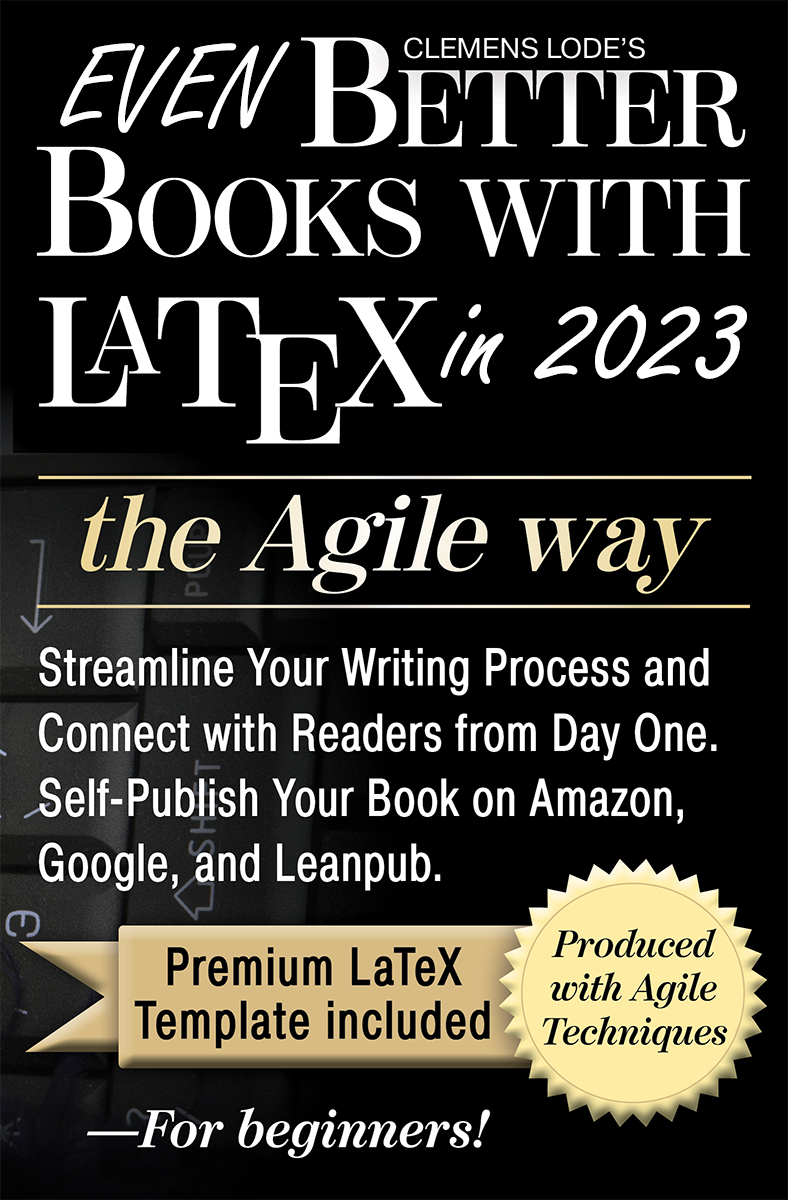
\includegraphics[width=.45\textwidth]{images/cover.jpg}
\end{center}

At LODE Publishing, we also publish works on science, philosophy, and project management. Check out \url{https://www.lode.de/publications} for a list. If you are interested in working with us to publish your book or if you are seeking advice on the next steps to take, contact us at \textbf{mail@lode.de}.

% %%%%%%%%%%%%%%%%%%%%%%%%%%%%%%%%%%%%%
% Check out the accompanying book, Even Better Books with LaTeX the Agile Way in 2023, for a discussion of the template and step-by-step instructions. https://amzn.to/3HqwgXM https://leanpub.com/eBBwLtAW/
% The template was originally created by Clemens Lode, LODE Publishing (www.lode.de), on 1/1/2023. Feel free to use this template for your book project!
% I would be happy if you included a short mention in your book in order to help others to create their own books, too ("Book template based on \textit{Even Better Books with LaTeX the Agile Way in 2023} by Clemens Lode").
% Contact me at mail@lode.de if you need help with the template or are interested in our editing and publishing services.
% And don't forget to follow us on Instagram! https://www.instagram.com/lodepublishing/ https://www.instagram.com/betterbookswithlatex/
%%%%%%%%%%%%%%%%%%%%%%%%%%%%%%%%%%%%%

% This file prints the author page.

% Upload a high-resolution (author_highres.png) and a low-resolution picture (author.jpg) of the author into the images folder and uncomment the 5 includegraphics lines.
% Replace the paragraph about quotations with a quotation of your choice.
% Add text describing your motivation, your professional background, what you are currently doing, and how to connect with you.

\chapter{The Author \yourName}
\label{the-author:cha}

\begin{center}

\ifuseAuthorImage
\ifxetex
	\includegraphics[width=.7\textwidth]{\authorImageHiRes}
\else
	\includegraphics{\authorImage}
\fi
\fi

\end{center}

\begin{myquotation} Here is space for a quotation that describes your journey through life (as opposed to just during the writing of this book). Pick one that best describes you, your attitude, or something you admire. Be personal!\end{myquotation}


Describe your dreams, what goals you have in life, where you went to school or studied, and what job you currently work or worked in the past. Make clear what motivated you to start writing. Finally, add contact points where people can connect with you (mail, Facebook, Instagram, TikTok, YouTube, Twitter, etc.).

% %%%%%%%%%%%%%%%%%%%%%%%%%%%%%%%%%%%%% 
% Check out the accompanying book, Even Better Books with LaTeX the Agile Way in 2023, for a discussion of the template and step-by-step instructions. https://amzn.to/3HqwgXM https://leanpub.com/eBBwLtAW/
% The template was originally created by Clemens Lode, LODE Publishing (www.lode.de), on 1/1/2023. Feel free to use this template for your book project! 
% I would be happy if you included a short mention in your book in order to help others to create their own books, too ("Book template based on \textit{Even Better Books with LaTeX the Agile Way in 2023} by Clemens Lode").
% Contact me at mail@lode.de if you need help with the template or are interested in our editing and publishing services.
% And don't forget to follow us on Instagram! https://www.instagram.com/lodepublishing/ https://www.instagram.com/betterbookswithlatex/
%%%%%%%%%%%%%%%%%%%%%%%%%%%%%%%%%%%%%

% Use this chapter to summarize what you have learned while writing the book. This helps you to write better books in the future, and it might be interesting for the reader to learn how the book came about.

\chapter{The Book's Story}\label{booksstory:cha}

% Add a quotation that encompasses or describes the lessons you learned while planning and writing the book.




% %%%%%%%%%%%%%%%%%%%%%%%%%%%%%%%%%%%%% 
% Check out the accompanying book, Even Better Books with LaTeX the Agile Way in 2023, for a discussion of the template and step-by-step instructions. https://amzn.to/3HqwgXM https://leanpub.com/eBBwLtAW/
% The template was originally created by Clemens Lode, LODE Publishing (www.lode.de), on 1/1/2023. Feel free to use this template for your book project! 
% I would be happy if you included a short mention in your book in order to help others to create their own books, too ("Book template based on \textit{Even Better Books with LaTeX the Agile Way in 2023} by Clemens Lode").
% Contact me at mail@lode.de if you need help with the template or are interested in our editing and publishing services.
% And don't forget to follow us on Instagram! https://www.instagram.com/lodepublishing/ https://www.instagram.com/betterbookswithlatex/
%%%%%%%%%%%%%%%%%%%%%%%%%%%%%%%%%%%%%

\chapter{Reflection}

\begin{problem}
Introductory text about what this section is about. For example, describe that this is a summary of all the ``problem boxes'' throughout the book and point to an online forum where readers can discuss them.\end{problem}

% If you would like to reset formatting, use this code.
\setlength{\parindent}{0.0cm}
\renewcommand{\index}[1]{}
\renewenvironment{problem}[1][]{$\bullet$\ #1}
\footnotesize 


\section*{Replace with Your First Chapter}
% Add questions encountered in your first chapter.
\begin{problem}What is LaTeX?\end{problem}


\section*{Replace with Your Second Chapter}
% Add questions encountered in your second chapter.

\section*{Replace with Your Third Chapter}
% Add questions encountered in your third chapter.
% \index{XeLaTeX@\textit{XeLaTeX}|textbf}
% %%%%%%%%%%%%%%%%%%%%%%%%%%%%%%%%%%%%% 
% Check out the accompanying book, Even Better Books with LaTeX the Agile Way in 2023, for a discussion of the template and step-by-step instructions. https://amzn.to/3HqwgXM https://leanpub.com/eBBwLtAW/
% The template was originally created by Clemens Lode, LODE Publishing (www.lode.de), on 1/1/2023. Feel free to use this template for your book project! 
% I would be happy if you included a short mention in your book in order to help others to create their own books, too ("Book template based on \textit{Even Better Books with LaTeX the Agile Way in 2023} by Clemens Lode").
% Contact me at mail@lode.de if you need help with the template or are interested in our editing and publishing services.
% And don't forget to follow us on Instagram! https://www.instagram.com/lodepublishing/ https://www.instagram.com/betterbookswithlatex/
%%%%%%%%%%%%%%%%%%%%%%%%%%%%%%%%%%%%%

% This file summarizes the conclusions or summaries of each chapter.

\chapter{Eureka!}

\begin{idea}
Introductory text about what this section is about. For example, describe that this is a summary of all the idea boxes throughout the book.\end{idea}

% Use the following command to reformat idea boxes.
\renewenvironment{idea}[1][]{$\bullet$\ #1}

% Use the following command to deactivate the indexing of idea boxes in order to prevent duplicates.
\ifxetex
        \renewcommand{\index}[1]{\ignorespaces}
\fi

\section*{Replace with Your First Chapter}
% Here, you can add ideas presented in your first chapter.
\begin{idea}
LaTeX is a document preparation system.
\end{idea}

\section*{Replace with Your Second Chapter}
% Here, you can add ideas presented in your second chapter.

\section*{Replace with Your Third Chapter}
% Here, you can add ideas presented in your third chapter.
% \index{XeLaTeX@\textit{XeLaTeX}|textbf}
% %%%%%%%%%%%%%%%%%%%%%%%%%%%%%%%%%%%%%
% Check out the accompanying book, Even Better Books with LaTeX the Agile Way in 2023, for a discussion of the template and step-by-step instructions. https://amzn.to/3HqwgXM https://leanpub.com/eBBwLtAW/
% The template was originally created by Clemens Lode, LODE Publishing (www.lode.de), on 1/1/2023. Feel free to use this template for your book project!
% I would be happy if you included a short mention in your book in order to help others to create their own books, too ("Book template based on \textit{Even Better Books with LaTeX the Agile Way in 2023} by Clemens Lode").
% Contact me at mail@lode.de if you need help with the template or are interested in our editing and publishing services.
% And don't forget to follow us on Instagram! https://www.instagram.com/lodepublishing/ https://www.instagram.com/betterbookswithlatex/
%%%%%%%%%%%%%%%%%%%%%%%%%%%%%%%%%%%%%

% This file lists the glossary items throughout the book.

% If you have added or removed any entries in the glossary directory, add them here. If a letter is missing, add a new \section*{} with the letter.

\chapter{Glossary}
\label{glossary:cha}

\section*{C}
\begin{multicols}{2}
\babelEN{\begin{definition}{Citavi} \textit{Citavi} is a plugin for Word (see \url{https://www.citavi.com}) to manage your bibliography and citations.\end{definition}}\index{Citavi@\textit{Citavi}|textbf}
\end{multicols}

\section*{L}
\begin{multicols}{2}
\begin{definition}{LaTeX}\index{latex|textbf} LaTeX is a document preparation system.\end{definition}
\end{multicols}

\section*{O}
\begin{multicols}{2}
\babelEN{\begin{definition}{Overleaf} \textit{Overleaf} is an online editor and project manager for LaTeX documents. It manages your project with a versioning system and automatically compiles your LaTeX code into PDF and (with some help) HTML. It is free for public projects and does not require installation or setup. You can get an account here: \url{https://www.overleaf.com}.\end{definition}}\index{Overleaf@\textit{Overleaf}|textbf}

\end{multicols}

\section*{P}
\begin{multicols}{2}
\begin{definition}{pdfLaTeX} \textit{pdfLaTeX} is a basic LaTeX typesetting engine that translates LaTeX documents directly into PDFs or HTML files (with the help of \textit{TeX4ht}).\end{definition}\index{pdfLaTeX@\textit{pdfLaTeX}|textbf}
\end{multicols}

\section*{V}
\begin{multicols}{2}
\begin{definition}{Versioning system} A \textit{versioning system} is a tool to track changes to a document. That means you can go back and check what has been changed and by whom.\end{definition}\index{versioning system|textbf}
\end{multicols}

\section*{W}
\begin{multicols}{2}
\begin{definition}{Word} \textit{Word} usually refers to \textit{Microsoft Word}. Generally, it is used as an umbrella term for all word processors that directly show you what you will get as an end result (as opposed to first having to process the file). This approach is intuitive, but it makes editing large projects very complicated.\end{definition}\index{Word@\textit{Word}|textbf}
\end{multicols}

\section*{X}
\begin{multicols}{2}
\begin{definition}{XeLaTeX} \textit{XeLaTeX} is a LaTeX typesetting engine with an extended font, as well as UTF-8 encoding (for special characters) support. It takes longer to compile with \textit{XeLaTeX} than with the more basic \textit{pdfLaTeX}.\end{definition}\index{XeLaTeX@\textit{XeLaTeX}|textbf}




\end{multicols}


% This adds a separate quotations page (sources in the e-book are already included in the text body).
% \ifxetex
%     %%%%%%%%%%%%%%%%%%%%%%%%%%%%%%%%%%%%%
% Check out the accompanying book, Even Better Books with LaTeX the Agile Way in 2023, for a discussion of the template and step-by-step instructions. https://amzn.to/3HqwgXM https://leanpub.com/eBBwLtAW/
% The template was originally created by Clemens Lode, LODE Publishing (www.lode.de), on 1/1/2023. Feel free to use this template for your book project!
% I would be happy if you included a short mention in your book in order to help others to create their own books, too ("Book template based on \textit{Even Better Books with LaTeX the Agile Way in 2023} by Clemens Lode").
% Contact me at mail@lode.de if you need help with the template or are interested in our editing and publishing services.
% And don't forget to follow us on Instagram! https://www.instagram.com/lodepublishing/ https://www.instagram.com/betterbookswithlatex/
%%%%%%%%%%%%%%%%%%%%%%%%%%%%%%%%%%%%%

% This file adds a page with quotation sources you have used in your book.

% This is displayed only for print PDFs where the source is not directly mentioned in the text body.

\chapter{Quotation Sources}

\setlength{\parindent}{0pt}
\footnotesize

\babelES{\textbf{\pageref{gogh-sky-quote}:} \cite[vgl.][S.~23--24]{ifyouwanttowrite}}
\babelEN{\textbf{\pageref{gogh-sky-quote}:} \cite[pp.~23--24]{ifyouwanttowrite}}\par

% \fi

% %%%%%%%%%%%%%%%%%%%%%%%%%%%%%%%%%%%%%
% Check out the accompanying book, Even Better Books with LaTeX the Agile Way in 2023, for a discussion of the template and step-by-step instructions. https://amzn.to/3HqwgXM https://leanpub.com/eBBwLtAW/
% The template was originally created by Clemens Lode, LODE Publishing (www.lode.de), on 1/1/2023. Feel free to use this template for your book project!
% I would be happy if you included a short mention in your book in order to help others to create their own books, too ("Book template based on \textit{Even Better Books with LaTeX the Agile Way in 2023} by Clemens Lode").
% Contact me at mail@lode.de if you need help with the template or are interested in our editing and publishing services.
% And don't forget to follow us on Instagram! https://www.instagram.com/lodepublishing/ https://www.instagram.com/betterbookswithlatex/
%%%%%%%%%%%%%%%%%%%%%%%%%%%%%%%%%%%%%

% This file prints the bibliography.

%  Uncomment the command below if you want to add a preface to the bibliography (between the title and the list of referenced books). See https://tex.stackexchange.com/questions/197061/text-between-index-or-bibliography-title-and-content

%\bibpreface {Add the preface of your list of recommended reading titles here. Delete this line to have no preface for this section.}

\ifxetex
    \printbibliography
\else
    \bibliographystyle{plainnat}
    \babelEN{\bibliography{chapters/bibliography/english}}
\fi


%%%%%%%%%%%%%%%%%
% Appendix
%%%%%%%%%%%%%%%%%
% \appendix

% The index page exists only for printed PDFs.
\ifxetex
    % This is an optional command to display a prologue before the index.
    % \indexprologue{Replace index prologue with an own introduction (errata, formatting, abbreviations, etc.).}

    \printindex
    \thispagestyle{empty}
\fi

% %%%%%%%%%%%%%%%%%%%%%%%%%%%%%%%%%%%%% 
% Check out the accompanying book, Even Better Books with LaTeX the Agile Way in 2023, for a discussion of the template and step-by-step instructions. https://amzn.to/3HqwgXM https://leanpub.com/eBBwLtAW/
% The template was originally created by Clemens Lode, LODE Publishing (www.lode.de), on 1/1/2023. Feel free to use this template for your book project! 
% I would be happy if you included a short mention in your book in order to help others to create their own books, too ("Book template based on \textit{Even Better Books with LaTeX the Agile Way in 2023} by Clemens Lode").
% Contact me at mail@lode.de if you need help with the template or are interested in our editing and publishing services.
% And don't forget to follow us on Instagram! https://www.instagram.com/lodepublishing/ https://www.instagram.com/betterbookswithlatex/
%%%%%%%%%%%%%%%%%%%%%%%%%%%%%%%%%%%%%

% This file adds a page reminding the reader to leave a review.

% Replace this with your own call to action or use the default text.
\chapter{An Important Final Note}

% Show this paragraph only for e-books.
\ifxetex \else \textit{If you want to rate this e-book, please also add a short text comment. Without a text comment, your star rating will be invisible on the Amazon website and count only as an indicator for additional recommendations on Amazon. Thanks!}\fi

% Show the following for e-books and printed books. 
Writers are not performance artists. While there are book signings and public readings, most writers (and readers) follow their passion alone in their homes.

\textit{What applause is for the musician, \textbf{reviews} are for the writer.} 

\textit{Books create a community among readers}; you can share your thoughts among all those who will or have read the book.

\textbf{Leave a thoughtful, honest review and help me to create such a community on the platform on which you have acquired this book.} 
\textit{What did you like, what can be improved? To whom would you recommend it?} 

Thank you, also in the name of all the other readers who will be able to better decide whether this book is right for them or not. A positive review will increase the reach of the book; a negative review will improve the quality of the next book. I welcome both!
% %%%%%%%%%%%%%%%%%%%%%%%%%%%%%%%%%%%%% 
% Check out the accompanying book, Even Better Books with LaTeX the Agile Way in 2023, for a discussion of the template and step-by-step instructions. https://amzn.to/3HqwgXM https://leanpub.com/eBBwLtAW/
% The template was originally created by Clemens Lode, LODE Publishing (www.lode.de), on 1/1/2023. Feel free to use this template for your book project! 
% I would be happy if you included a short mention in your book in order to help others to create their own books, too ("Book template based on \textit{Even Better Books with LaTeX the Agile Way in 2023} by Clemens Lode").
% Contact me at mail@lode.de if you need help with the template or are interested in our editing and publishing services.
% And don't forget to follow us on Instagram! https://www.instagram.com/lodepublishing/ https://www.instagram.com/betterbookswithlatex/
%%%%%%%%%%%%%%%%%%%%%%%%%%%%%%%%%%%%%
% This file is the last page of the book.

\thispagestyle{empty}
\ifxetex
    \vspace*{\fill}
\fi
\hfill

% Replace the quote.
\babelEN{\begin{myquotation} Replace this quote\par\mbox{}\hfill \emdash{}Name of the author\end{myquotation}}

\end{document}
